\documentclass{article}
\usepackage[utf8]{inputenc}

\title{IIA Unipi - 2 Parte}
\author{Raffaele Apetino}
\date{March 2020}

\usepackage{natbib}
\usepackage{graphicx}
\usepackage[margin=3cm]{geometry}
\usepackage{amssymb}
\usepackage{xcolor}
\usepackage{proof}
\usepackage{float}

\begin{document}

\maketitle

\tableofcontents{}
\clearpage

\section{Giochi con avversario}
Il modello base a cui ci siamo affidati fin'ora è realizzato su ambienti osservabili, deterministici e con utente singolo.
I giochi con avversario invece si basano su ambienti deterministici multi-agente competitivo, in particolare su un ambiente reso strategico a causa della presenza di un avversario. Lo stato è più difficile da rappresentare e ha una struttura fattorizzata, nei sistemi basati su conoscenza lo stato è una "base di conoscenza" a cui rivolgere domande sul mondo rappresentato in un linguaggio espressivo, per poi essere gestite attraverso il PROP (calcolo proposizionale) o FOL (logica del primo ordine). 

\subsection{Ciclo Pianifica-Agisci-Percepisci}
Ci troviamo nel caso iun cui abbiamo due agenti che agiscono a turno, si pianifica considerando le possibili risposte dell'avversario e le risposte alla possibile risposta e così via. Una volta decisa la mossa migliore da fare, si agisce e si percepisce la mossa dell'avversario, infine si ripianifica la mossa. La decisione ottima teorica è definita come la mossa migliore in un gioco con uno spazio di ricerca completamente esplorabile (Algoritmo MinMax). E' possibile che ci troveremo in situazioni in cui a causa della complessità non sarà possibile eseguire una esplorazione esaustiva allora sfrutteremo tecniche di ottimizzazione della ricerca (Algoritmo ALFA-BETA).

\subsection{Definizione spazio degli stati}

\begin{itemize}
    \item Stati: configurazioni del gioco
    \item Stato iniziale: configurazione iniziale del gioco
    \item Player(s): a chi tocca eseguire l'azione nello stato s
    \item Action(s): mosse legali in s
    \item Result(s,a): stato risultante dopo aver eseguito la mossa a
    \item Terminal-Test(s): determina la fine del gioco, controlla che s sia lo stato terminale
    \item Utility(s,p): funzione di utilità (o pay-off) che resituisce un valopre numerico che valuta gli stati terminali del gioco per p (ad esempio somma di punteggi ecc...)
\end{itemize}
\newpage
\subsection{Algoritmo MinMax}
\begin{figure}[h!]
\centering
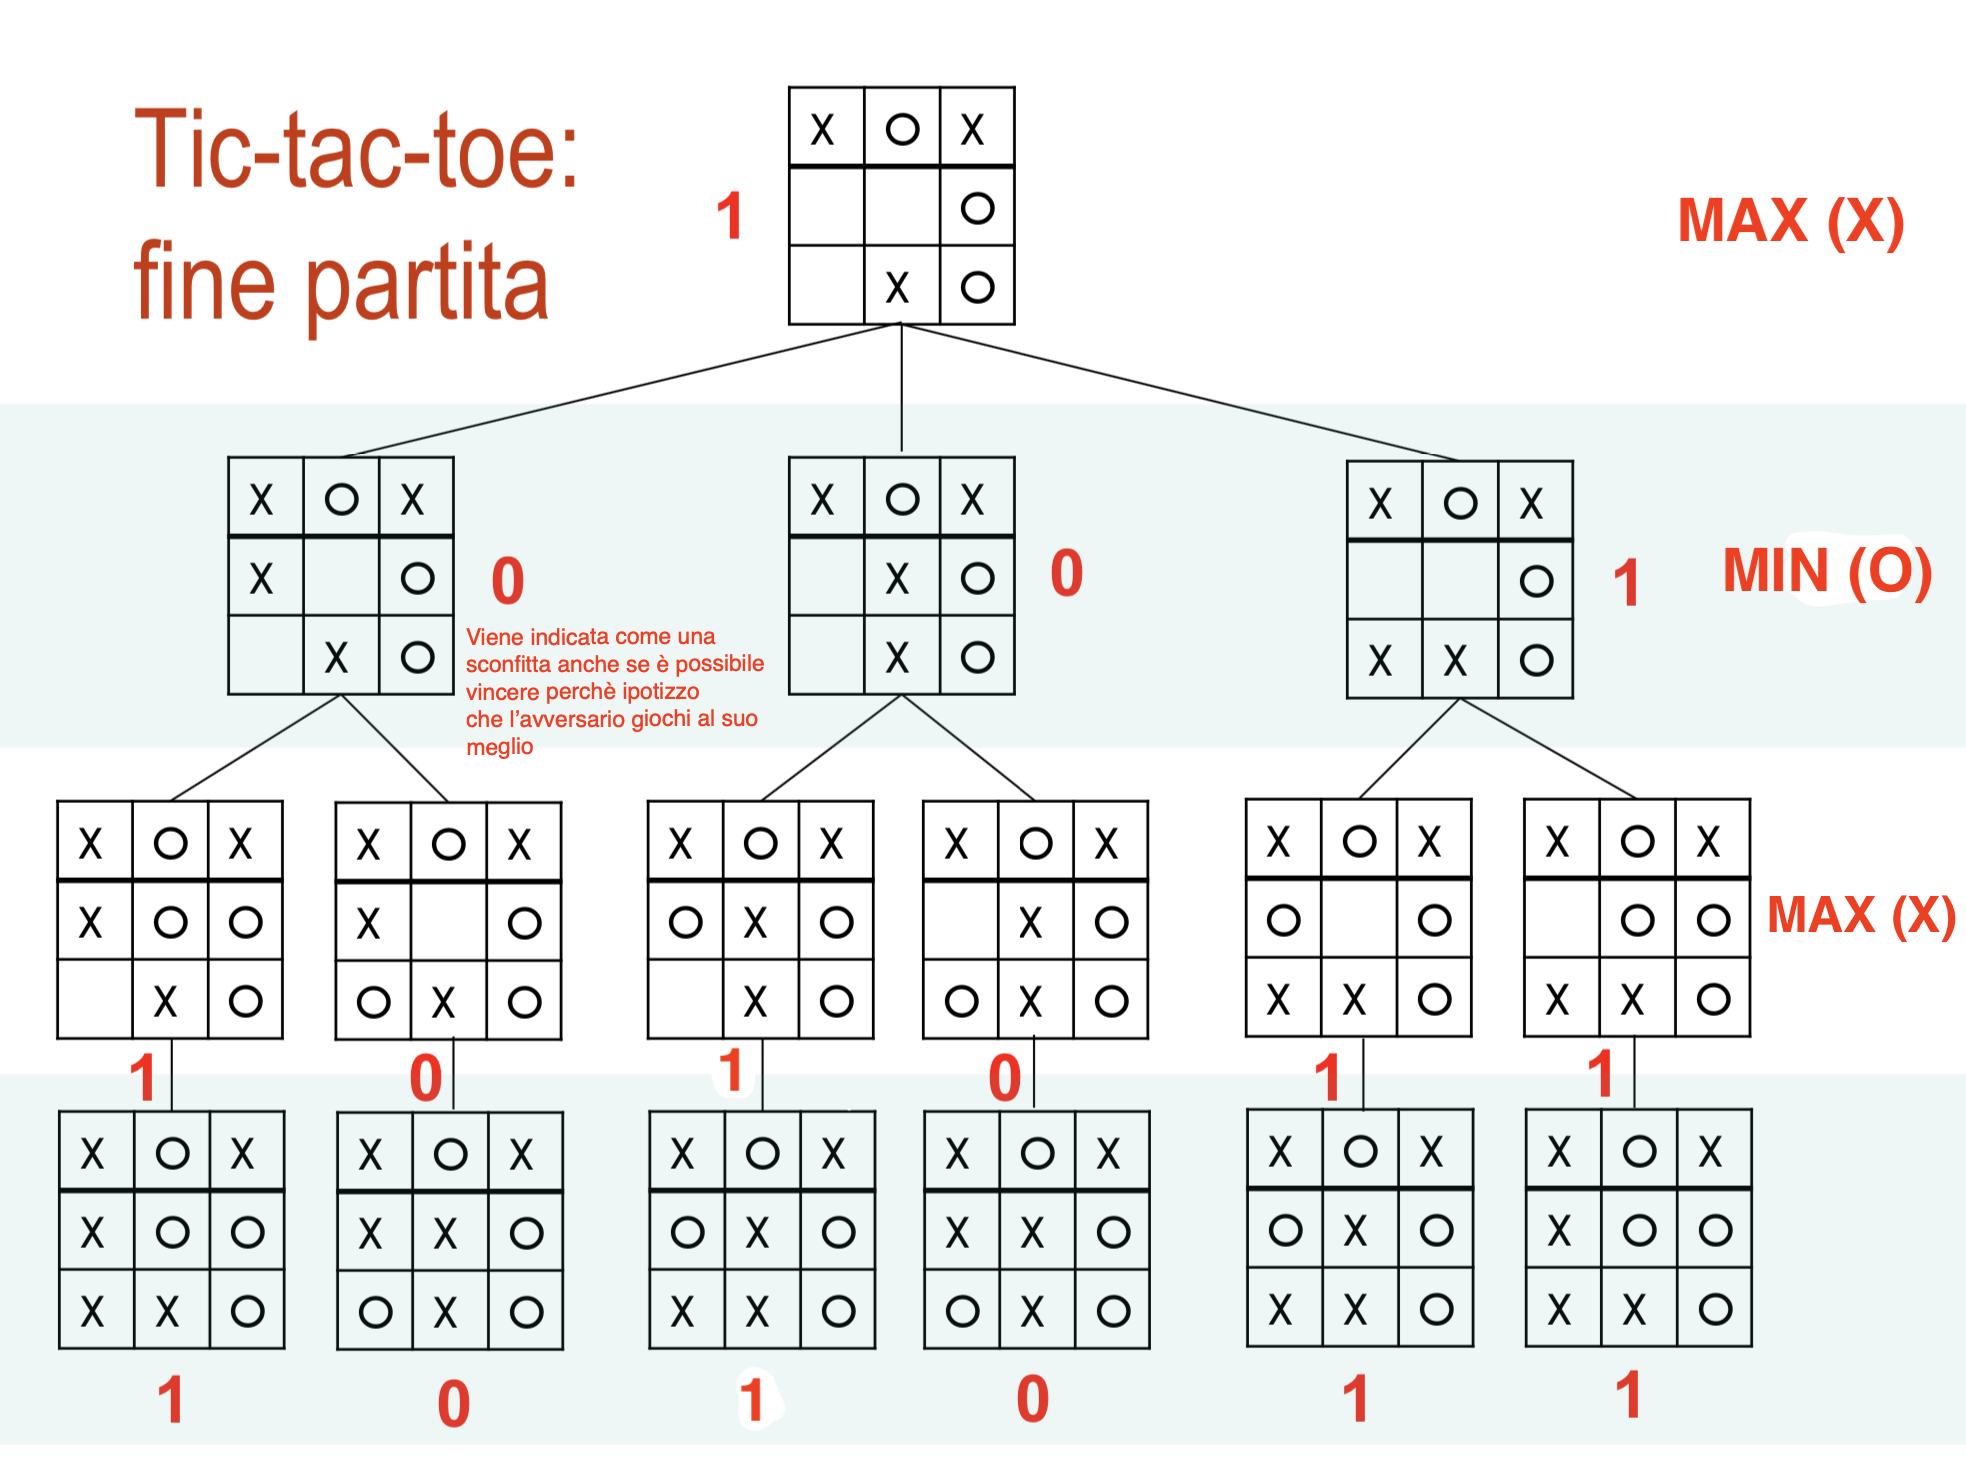
\includegraphics[scale=0.45]{Images/minmaxtictactoe.png}
\caption{The Universe}
\end{figure}

\subsubsection{Come si calcola il valore MinMax?}
MinMax(s) =
\begin{itemize}
    \item if (Terminal-Test(s) == true) Utility(s,MAX)
    \item if (Player(s) == MAX) max(MinMax(Result(s,a))) per ogni a $\in$ Actions(s)
    \item if (Player(s) == MIN) min(MinMax(Result(s,a))) per ogni a $\in$ Actions(s)
\end{itemize}
esplorando il grado in profondità perchè in ampiezza occuperei troppa memoria e a me interessa trovare uno dei tanti percorsi di vincita.
\newpage
\begin{figure}[h!]
\centering
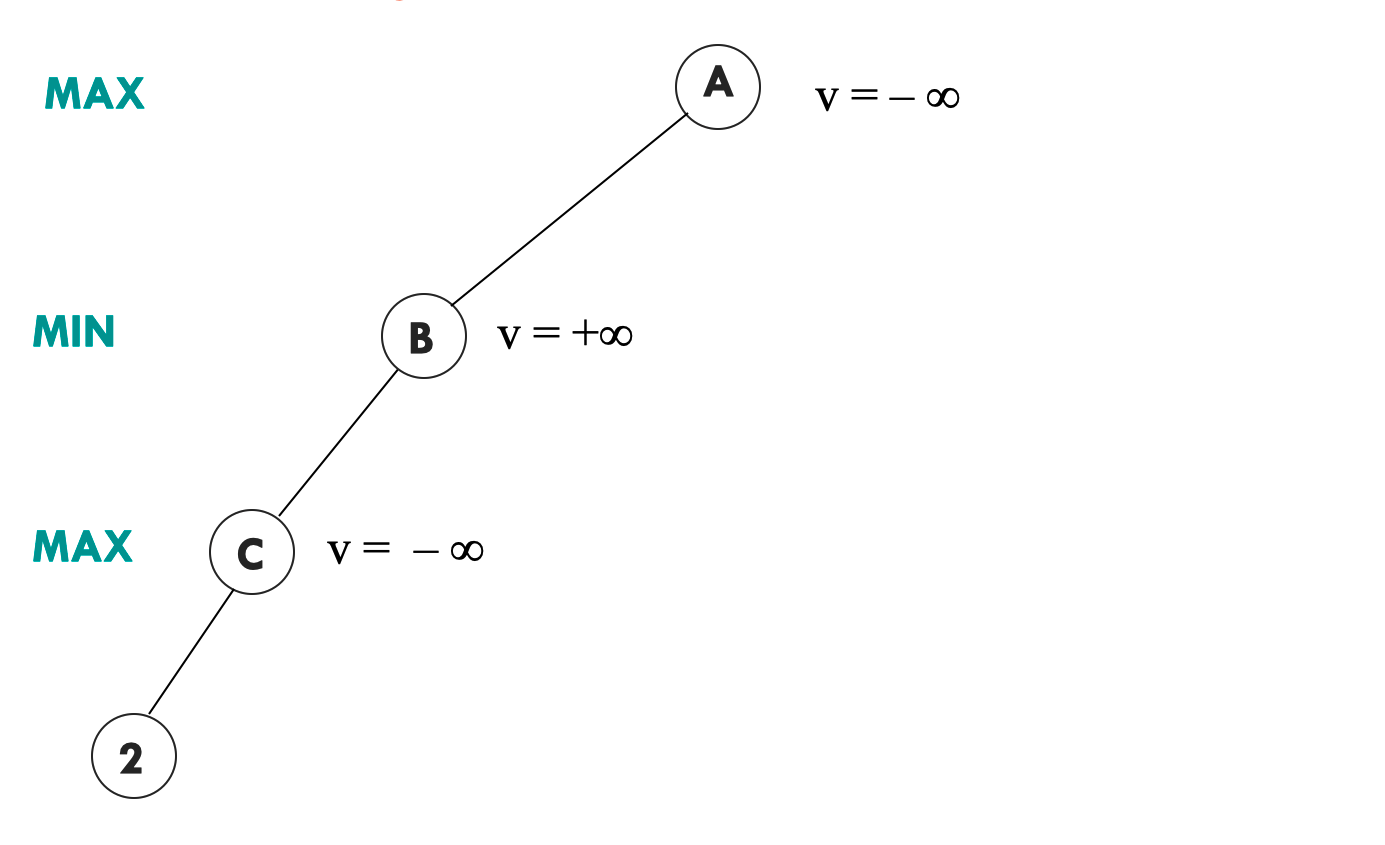
\includegraphics[scale=0.15]{Images/minmaxaction1.png}
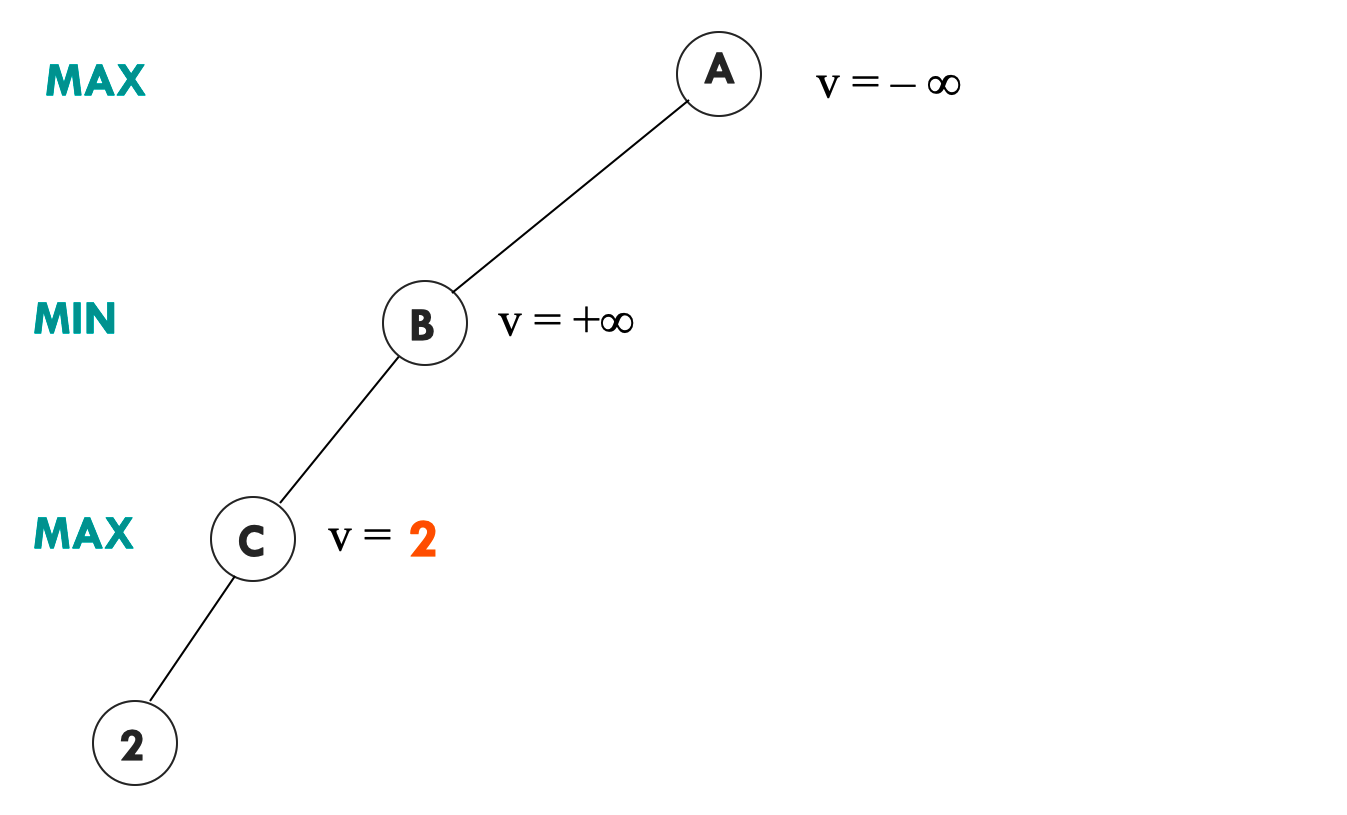
\includegraphics[scale=0.15]{Images/minmaxaction2.png}
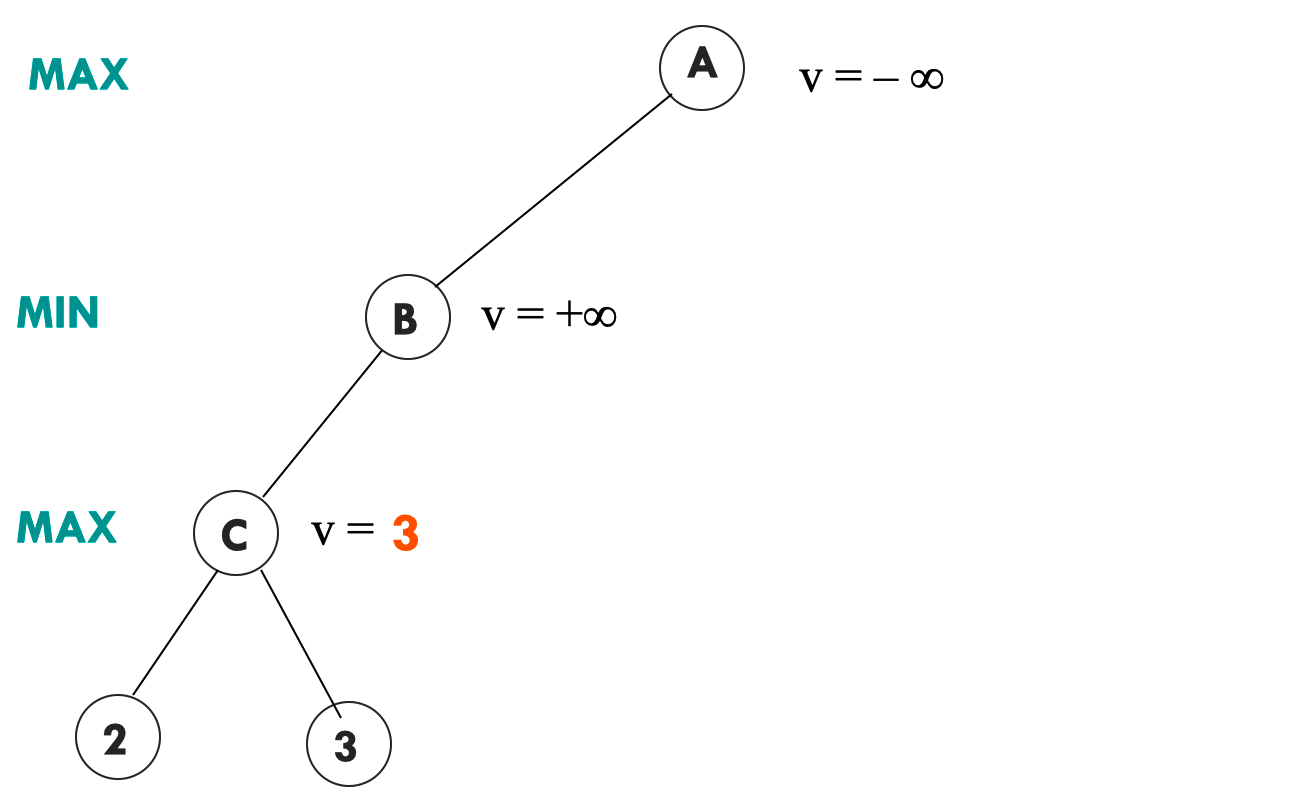
\includegraphics[scale=0.15]{Images/minmaxaction3.png}
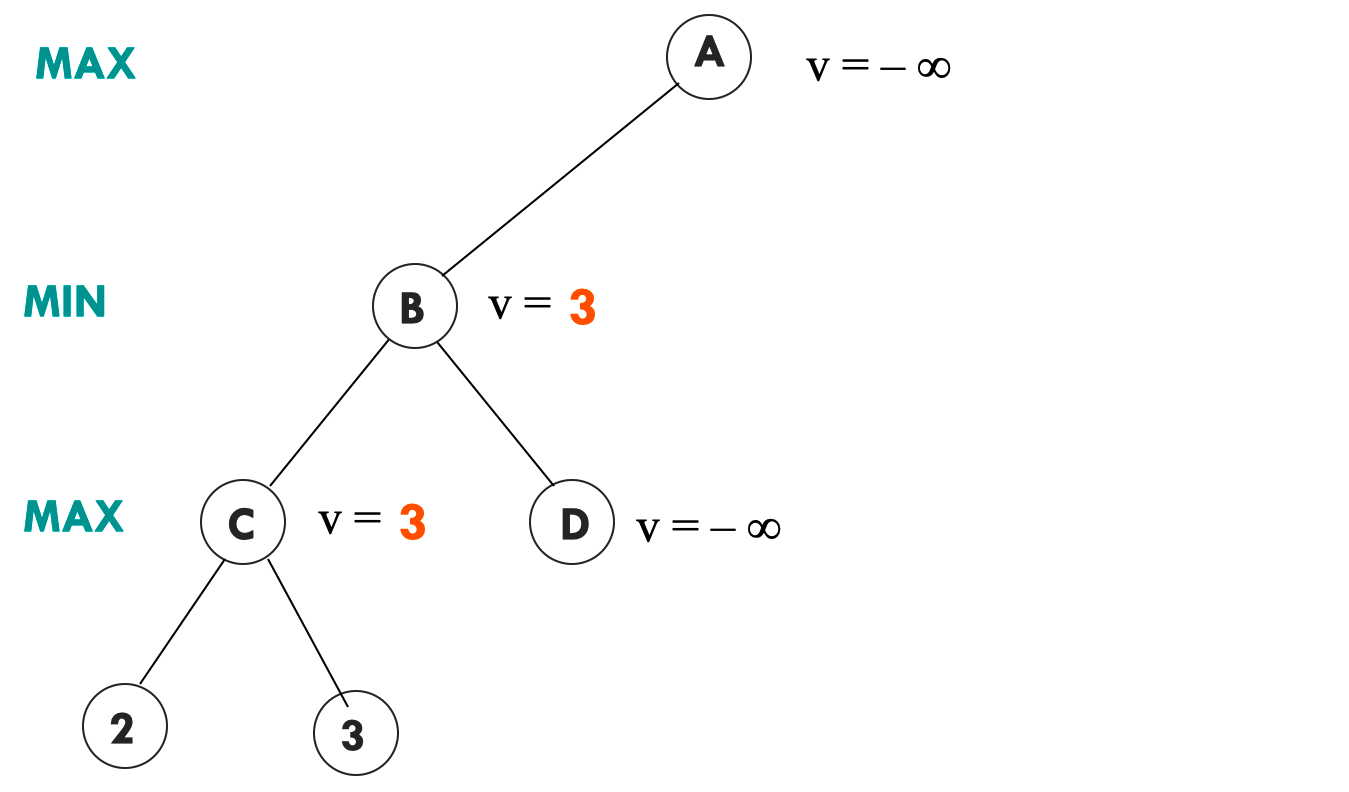
\includegraphics[scale=0.15]{Images/minmaxaction4.png}
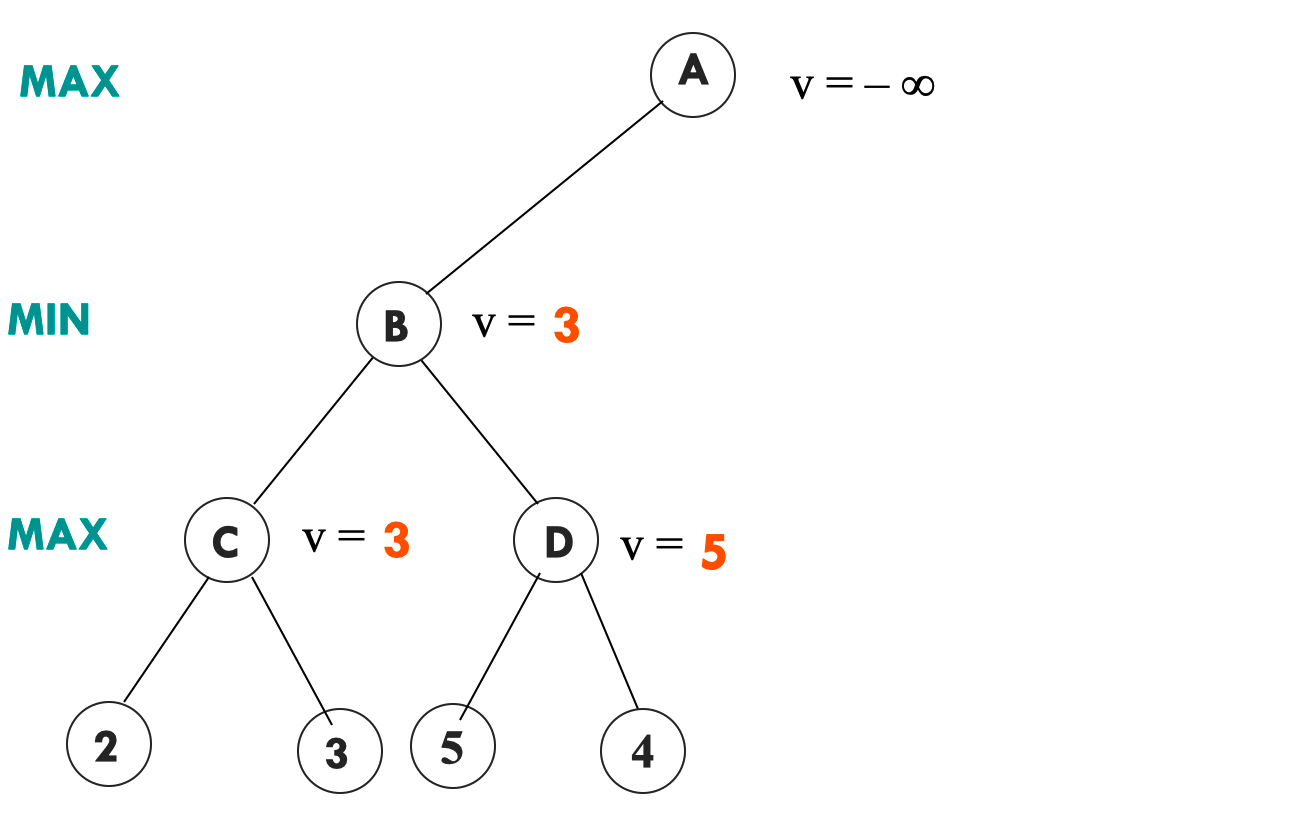
\includegraphics[scale=0.15]{Images/minmaxaction5.png}
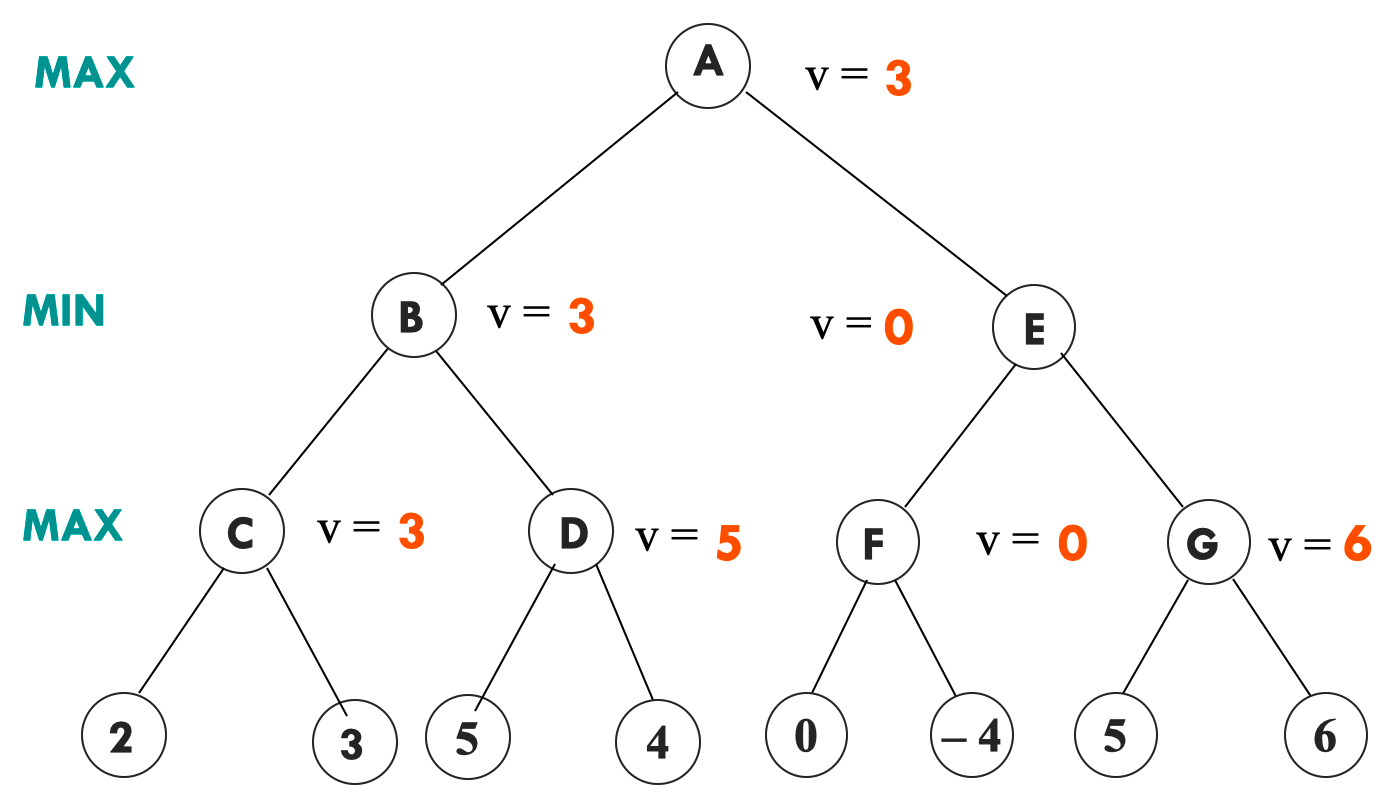
\includegraphics[scale=0.15]{Images/minmaxaction6.png}
\caption{Algoritmo MinMax in azione}
\end{figure}
\subsubsection{Costo MinMax}
\begin{itemize}
    \item Tempo: $O(b^m)$
    \item Spazio: $O(m)$
\end{itemize}
Si può notare come in giochi complessi come gli scacchi si abbia complessità in tempo di $O(35^{50})$ (35 mosse in media, 50 mosse per player) ottenendo un grafo di $(10^{40})$ nodi! Improponibile una esplorazione sistematica del grafo degli stati, se non per giochi veramente semplici. Troviamo quindi la necessità di far uso di euristiche per stimare il valore di uno stato del gioco.

\subsection{MinMax euristico (con orizzonte)}
Nei casi più complessi quindi occorre usare una funzione di valutazione euristica dello stato Eval(s). La strategia che applicheremo sarà quella di espandere l'albero di ricerca un certo numero di "d" livelli, si valutano gli stati ottenuti e si propaga indietro il risultato con la regola del MinMax.
\subsubsection{Come si calcola il valore MinMax euristico?}
H-MinMax(s,d) =
\begin{itemize}
    \item if (CutOff-Test(s,d) == true) Eval(s)
    \item if (Player(s) == MAX) max(H-MinMax(Result(s,a), d+1)) per ogni a $\in$ Actions(s)
    \item if (Player(s) == MIN) min(H-MinMax(Result(s,a), d+1)) per ogni a $\in$ Actions(s)
\end{itemize}
\subsubsection{Esempio MinMax euristico}
Usiamo come funzione di valutazione la differenza di "X(s)" righe aperte per X e "O(s)" righe aperte per O: \quad Eval(s) = X(s) - O(s) \\ La funzione di valutazione è una stima dell'utilità attesa a partire da una certa posizione nel gioco. La qualità della funzione è fondamentale: deve essere consistente con l'utilità se applicata a stati terminali del gioco, deve essere efficiente da calcolare (giochi a tempo) e deve riflettere le probabilità di vittoria.
\begin{figure}[h!]
\centering
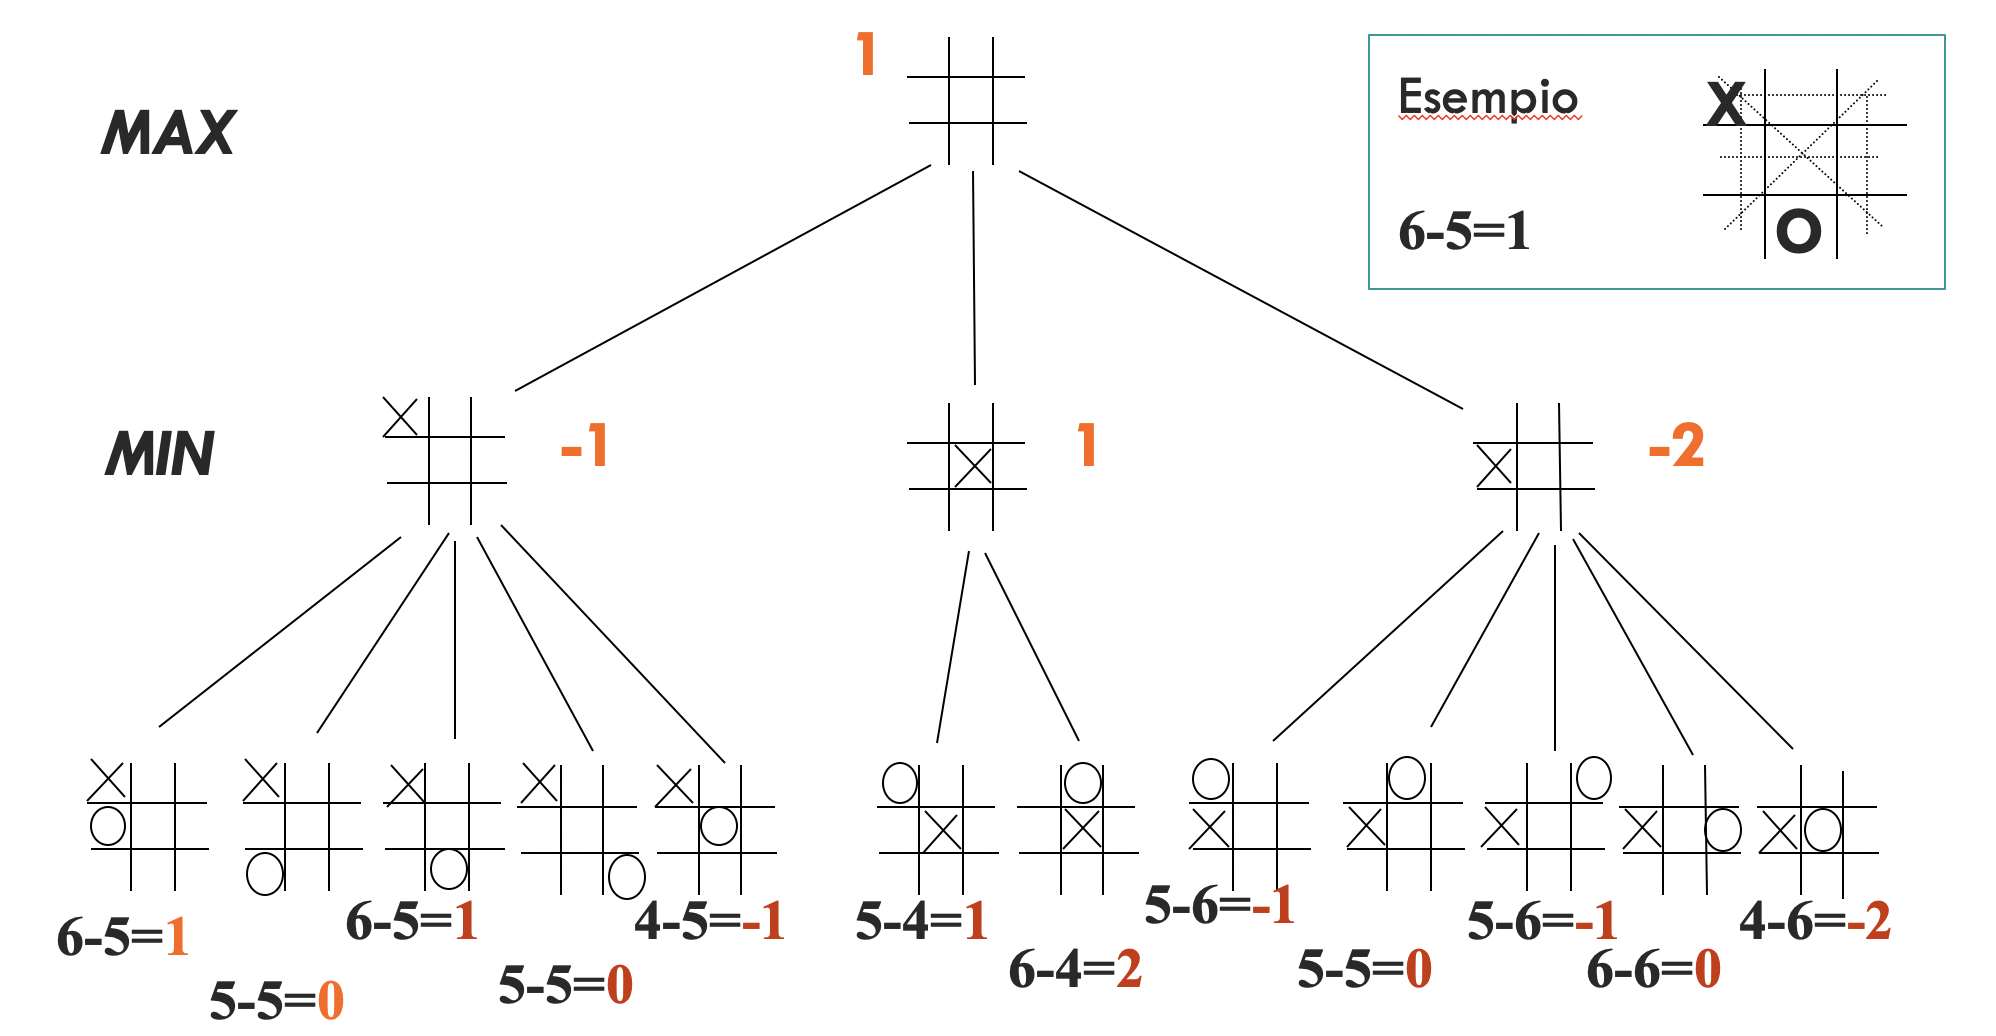
\includegraphics[scale=0.4]{Images/minmaxeuristico.png}
\caption{Algoritmo MinMax euristico in azione}
\end{figure}

\subsection{Problemi con MinMax}
\subsubsection{Stati non quiescienti}
L’esplorazione fino ad un livello può mostrare una situazione molto vantaggiosa ma alla mossa successiva la situazione può peggiorare esponenzialmente. La soluzione è applicare la valutazione a stati quiescenti, cioè stati in cui la funzione di valutazione non è soggetta a mutamenti repentini (questo implica la ricerca di quiescenza).
\subsubsection{Effetto orizzonte}
Può succedere che vengano privilegiate mosse diversive che hanno il solo effetto di spingere il problema oltre l’orizzonte. Una sorta di serie di mosse che non fanno altro che "scappare" dal problema il più possibile, magari ritrovandosi in un loop infinito.
\subsection{Ottimizzazione MinMax}
E' necessario esplorare ogni cammino? NO! si può sfruttare un metodo per dimezzare la ricerca pur mantenendo una decisione della prossima mossa corretta. (Potatura Alfa-Beta)
\subsection{Potatura Alfa-Beta}
E' una tecnica di potatura per ridurre l’esplorazione dello spazio di ricerca in algoritmi MinMax. L'idea è che si vada avanti in profondità fino al livello desiderato, si propaghi indietro i valori e a questo punto si decida se si può abbandonare l’esplorazione nel sotto-albero.
Sfruttiamo due valori "MaxValue" ($\alpha$) e "MinValue" ($\beta$) rispettivamente inizializzati a $\alpha=-\infty$ e $\beta=+\infty$. Rappresentano rispettivamente la migliore alternativa per MAX e per MIN fino a quel momento. \\
I tagli avvengono quando nel propagare indietro troviamo: 
\begin{itemize}
    \item $v \geq \beta$ per i nodi MAX (taglio $\beta$)
    \item $v \leq \alpha$ per i nodi MIN (taglio $\alpha$) 
\end{itemize}
\begin{figure}[h!]
\centering
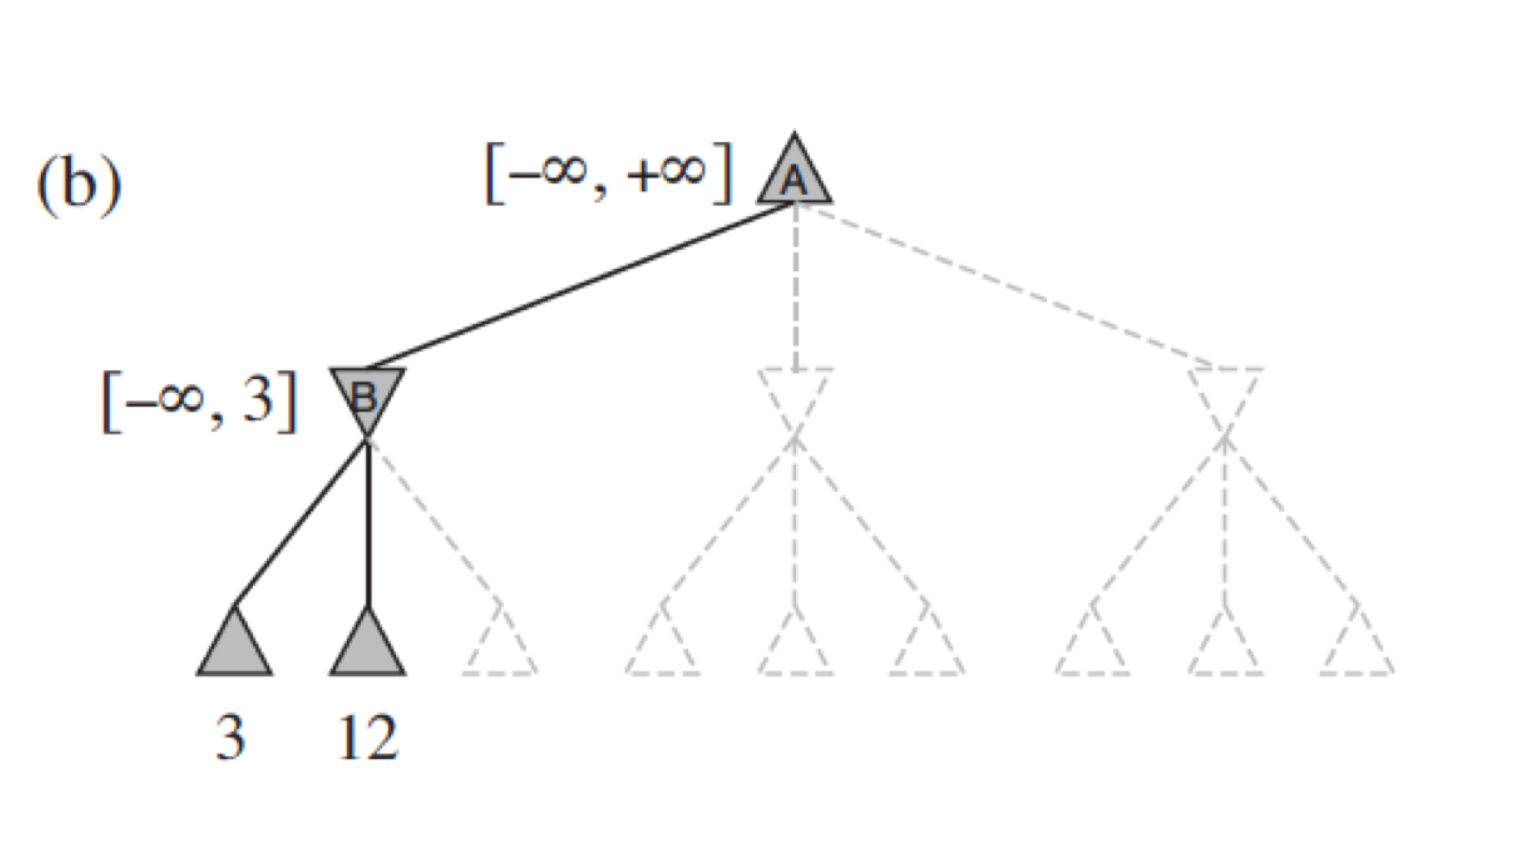
\includegraphics[scale=0.2]{Images/alfabetaaction1.png}
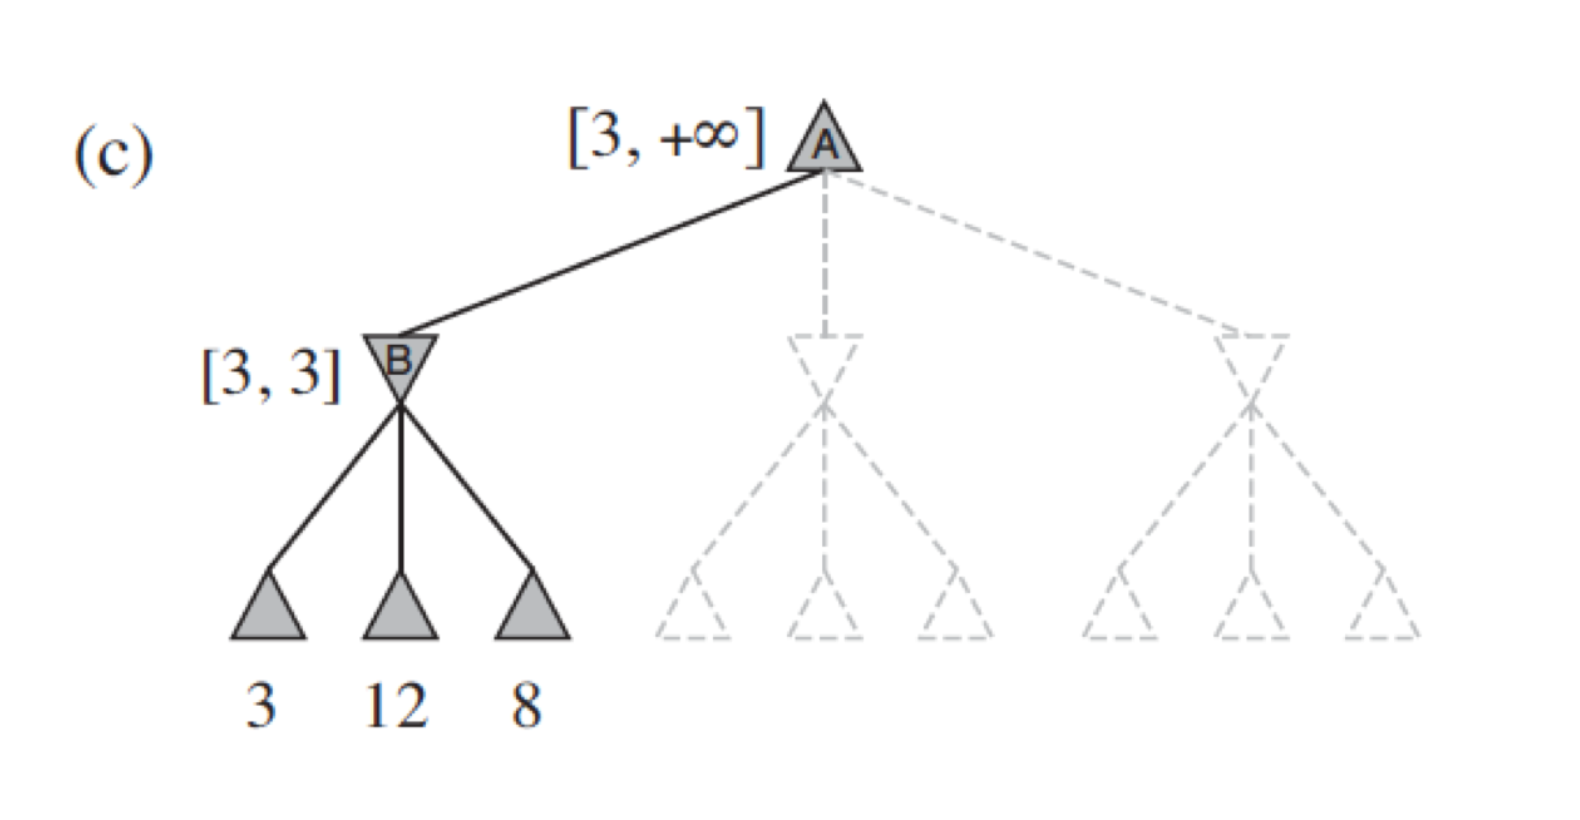
\includegraphics[scale=0.2]{Images/alfabetaaction2.png}
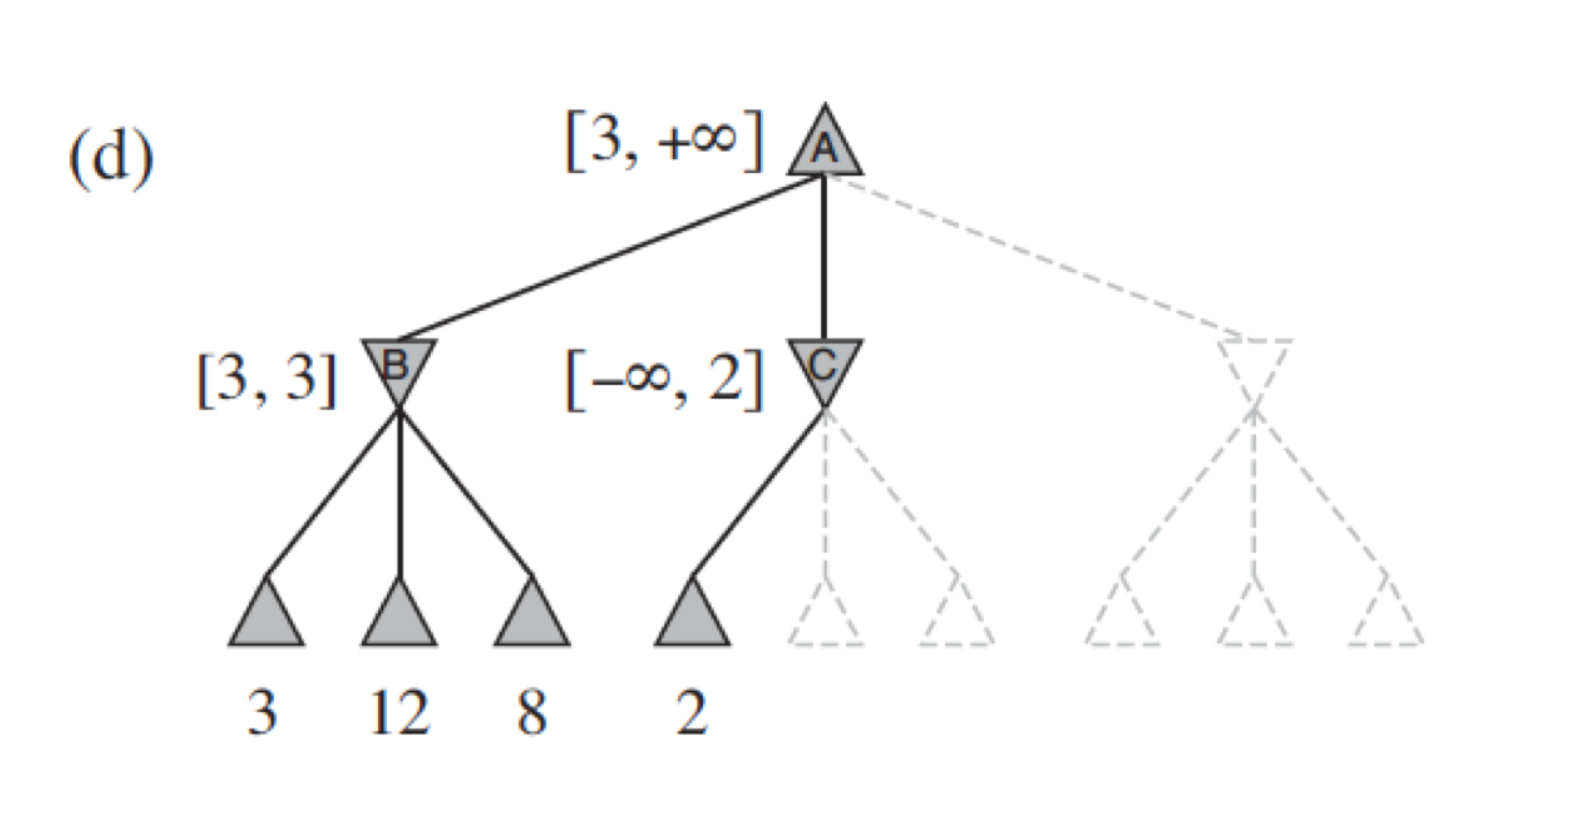
\includegraphics[scale=0.2]{Images/alfabetaaction3.png}
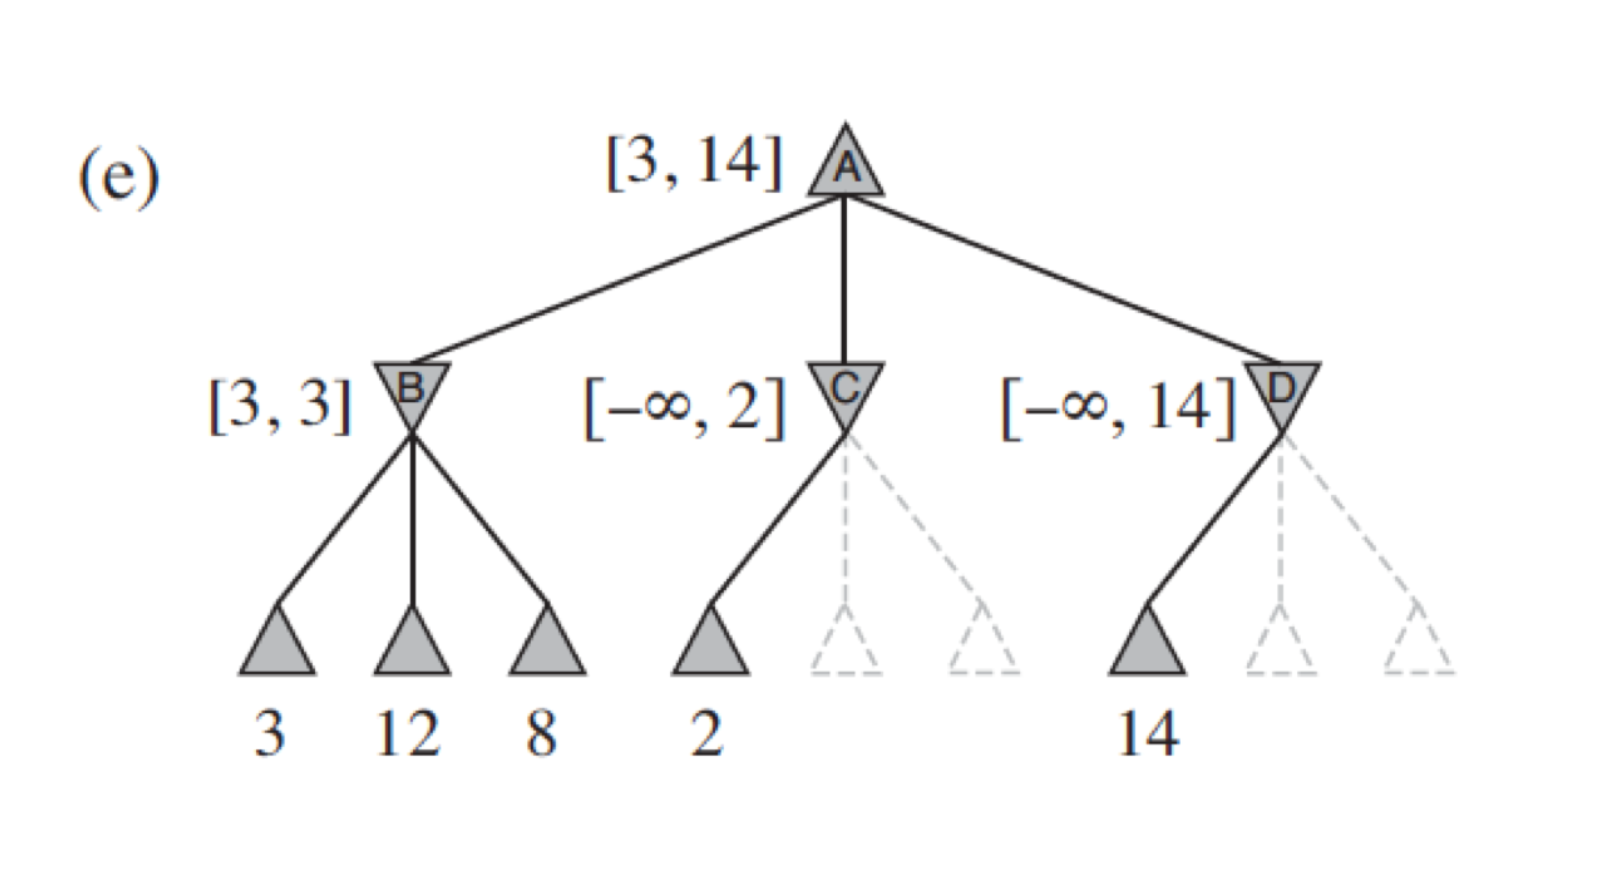
\includegraphics[scale=0.2]{Images/alfabetaaction4.png}
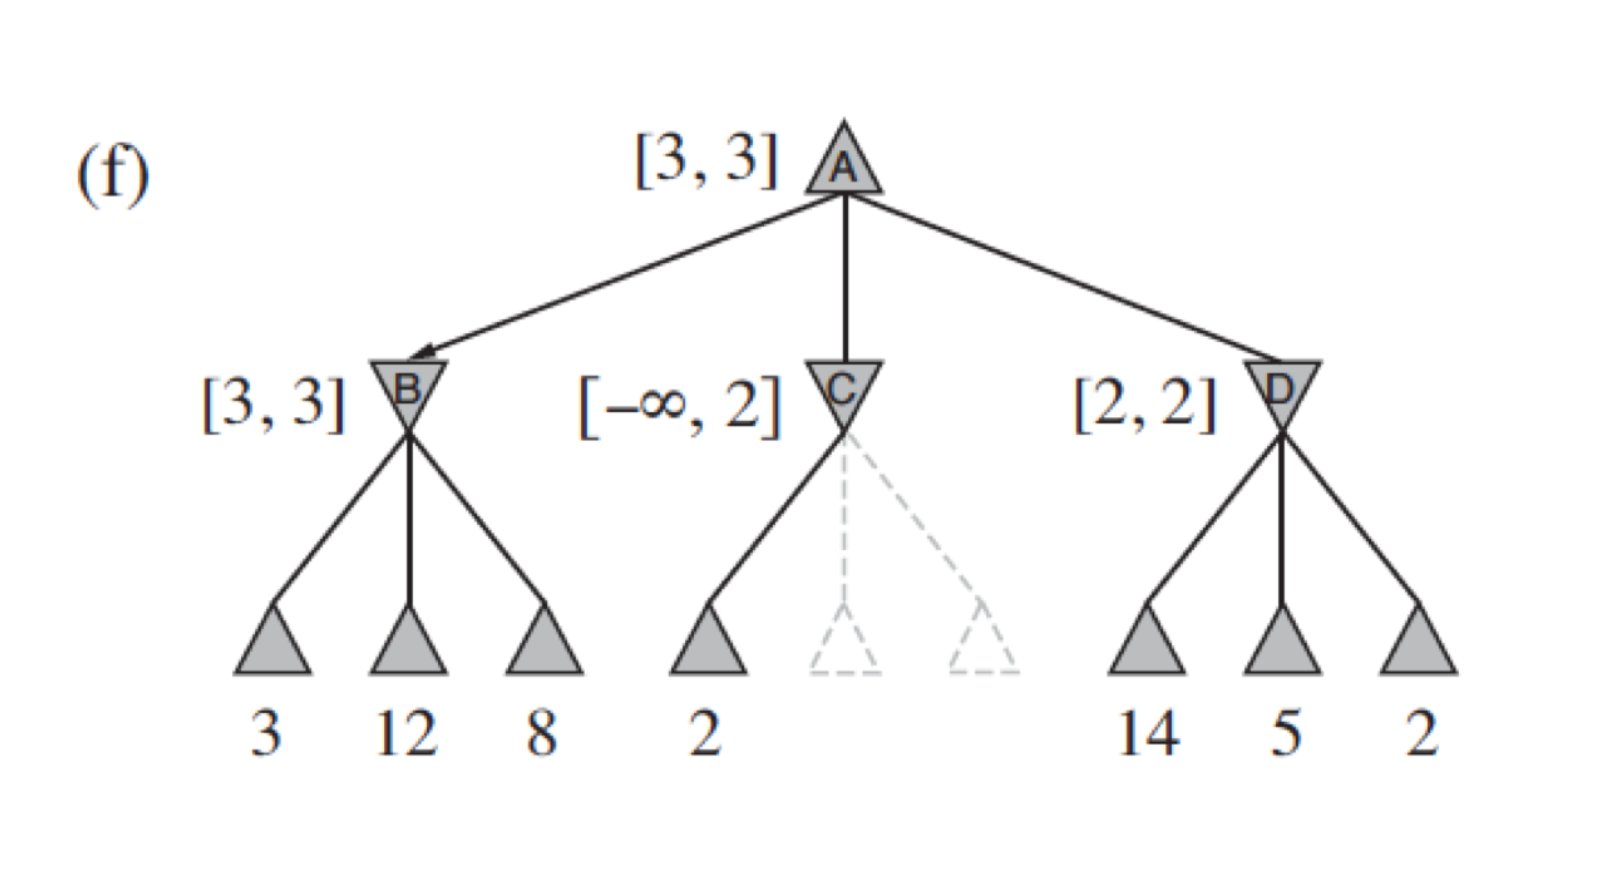
\includegraphics[scale=0.2]{Images/alfabetaaction5.png}
\caption{Potatura Alfa-Beta in azione}
\end{figure}
\subsubsection{Costo Potatura Alfa-Beta}
\begin{itemize}
    \item Tempo: $O(b^{m/2})$ quindi Alfa-Beta può arrivare a profondità doppia rispetto a MinMax (best case)
    \item Spazio: $O(m)$
\end{itemize}
\subsection{Ottimizzazioni Alfa-Beta}
Quale potrebbe essere l'ordinamento ottimale? Usando approfondimento iterativo si possono scoprire informazioni utili per l’ordinamento delle mosse da usare in una successiva iterazione. Teniamo conto a una  tabella delle trasposizioni: per ogni stato incontrato si memorizza la sua valutazione.
Si potrebbe anche eseguire una potatura in avanti, cioè esplorare solo alcune mosse ritenute promettenti e tagliare le altre (tagli probabilistici basati su esperienza). Possiamo inoltre sfruttare un database di mosse di apertura e chiusura: nelle prime fasi ci sono poche mosse sensate e ben studiate, inutile esplorarle tutte, mentre per le fasi finali il computer può esplorare off-line in maniera esaustiva e ricordarsi le migliori chiusure.
\subsubsection{Giochi Multiplayer}
Vengono valutati allo stesso tempo valori per ogni singolo giocatore.
\begin{figure}[h!]
\centering
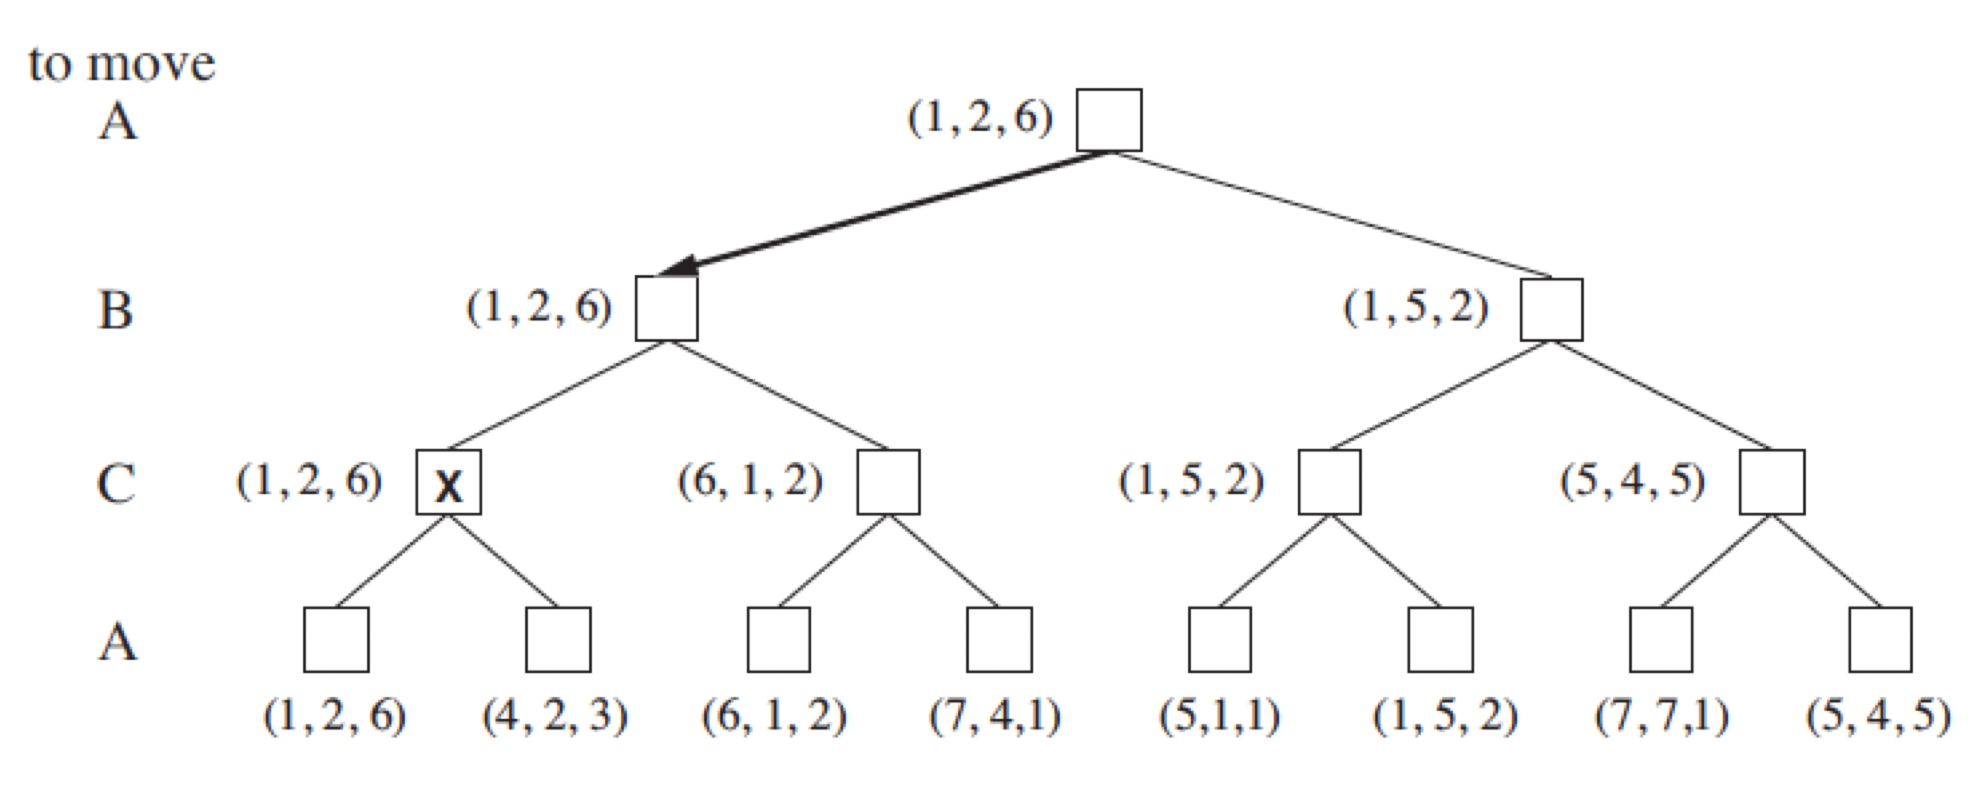
\includegraphics[scale=0.3]{Images/giochimultiplayer.png}
\caption{Giochi Multiplayer}
\end{figure}
\subsubsection{Giochi Complessi}
Giochi stocastici: i giochi in cui è previsto un lancio di dadi oppure la distribuzione di carte
Giochi parzialmente osservabili: le mosse sono deterministiche ma non si conoscono gli effetti delle mosse dell’avversario. (Battaglia navale)
\section{Problemi di soddisfacimento di vincoli (CSP)}
Sono problemi con una struttura particolare che necessitano algoritmi di ricerca specializzati. Con la rappresentazione fattorizzata dello stato si rende esplicita la struttura dello stato (o almeno in parte). Esistono euristiche generali che si applicano e che consentono la risoluzione di problemi di dimensioni significative per questa classe.
\subsection{Formulazione di problemi CSP}
\begin{itemize}
    \item Problema: descritto da tre componenti
        \begin{enumerate}
        \item X insieme di variabili
        \item D insieme di domini
        \item C insieme di vincoli
        \end{enumerate}
    \item Stato: un assegnamento parziale o completo di valori a variabili (ad esempio $X_i = v_i, X_j = v_j$ ecc...)
    \item Stato iniziale: {}
    \item Azioni: assegnamento valore ad una variabile
    \item Soluzione: un assegnamento completo della formula dove tutte le variabile hanno un valore e che sia consistente, cioè dove tutti i vincoli siano soddisfatti.
\end{itemize}
\subsection{Colorazione di una mappa}
\begin{figure}[h!]
\centering
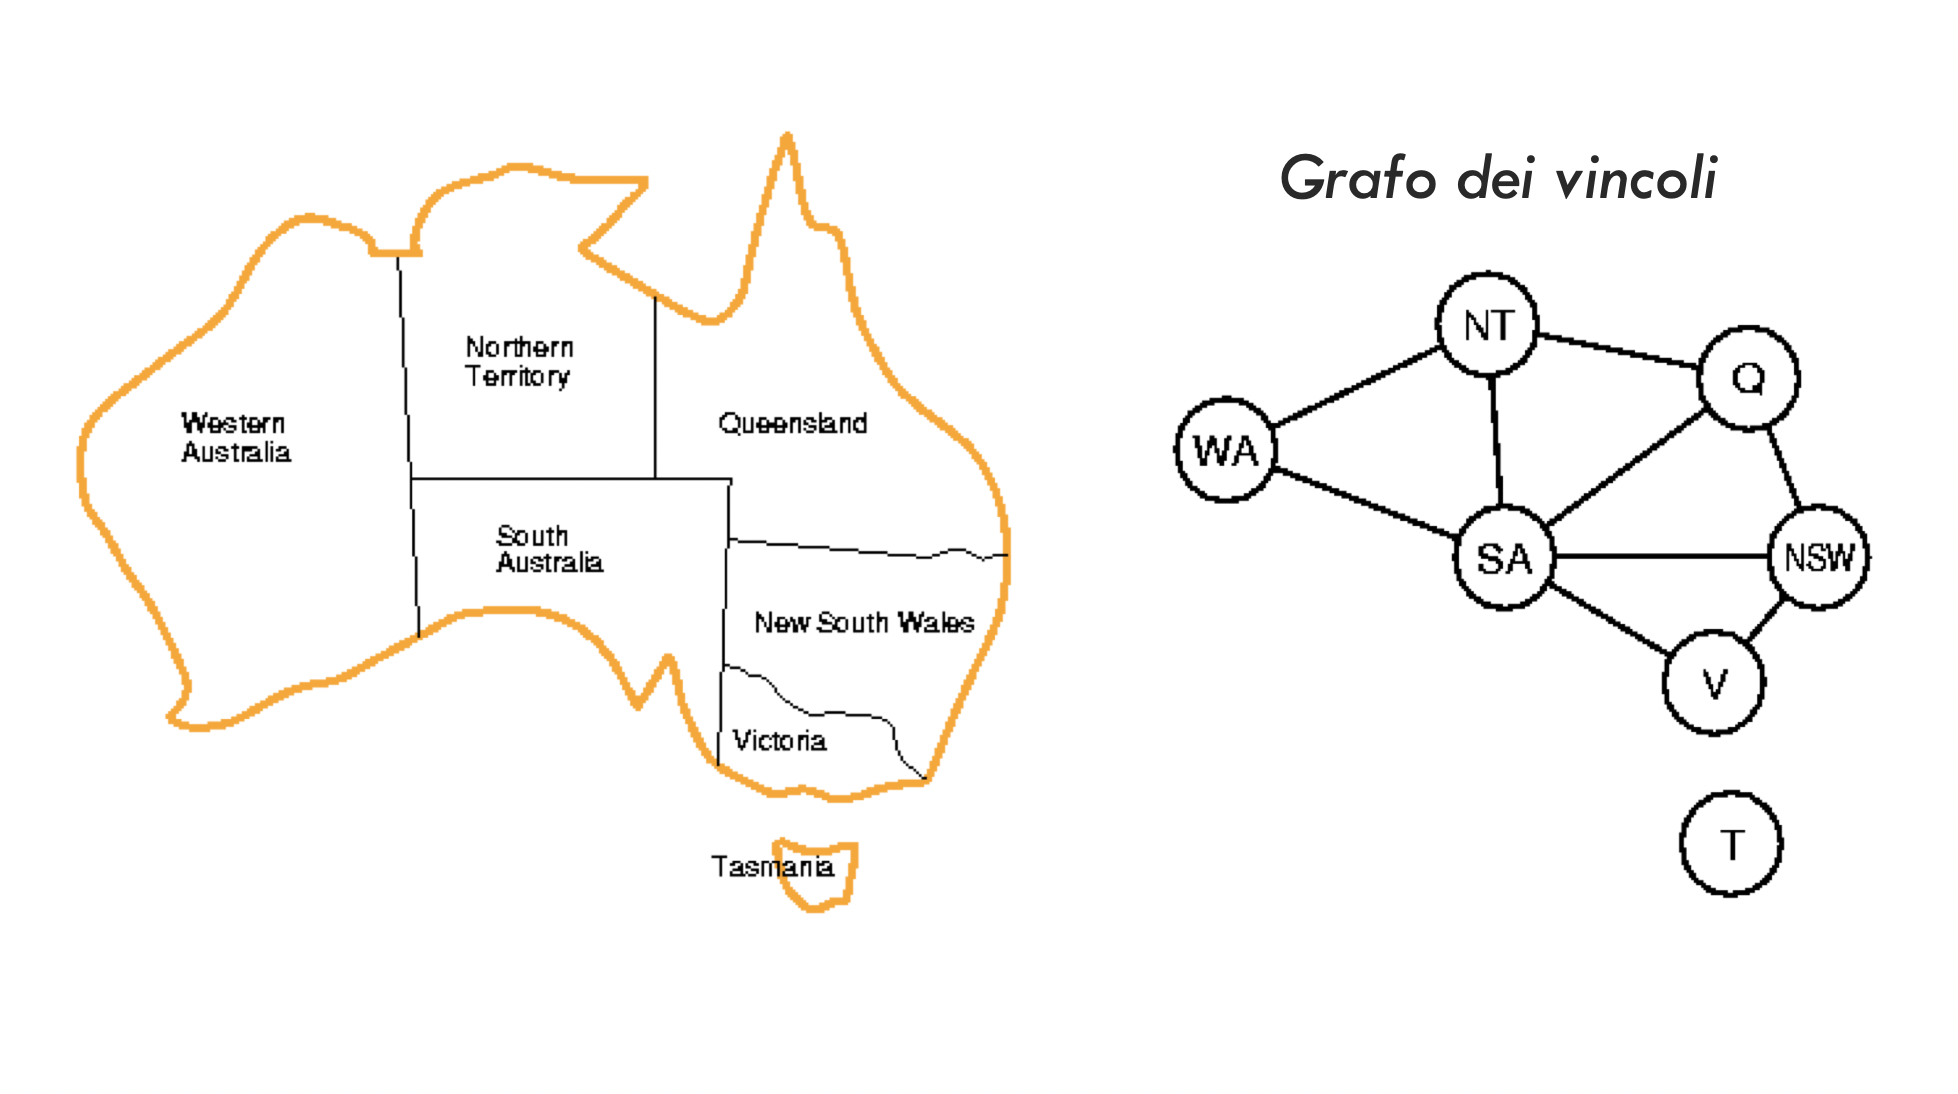
\includegraphics[scale=0.4]{Images/mappacolorata.png}
\caption{Problema colorazione mappa}
\end{figure}
Problema: Si tratta di colorare i diversi paesi sulla mappa con tre colori in modo che paesi adiacenti abbiano colori diversi.
\begin{enumerate}
    \item X = (WA, NT, SA, Q, NSW, V, T)
    \item $D_{WA} = D_{NT} = D_{SA} = D_Q = D_{NSW} = D_{V} = D_T$ = (red, green, blue)
    \item C = ($WA \neq NT, WA \neq SA, NT \neq Q, SA \neq Q, SA \neq NSW, SA \neq V, NSV \neq V$)
\end{enumerate}
\subsection{Problema 8 regine}
Problema: Si tratta di posizionare le 8 regine sulla scacchiera senza che nessuna sia in grado di mangiare un'altra.
\begin{enumerate}
    \item X = ($Q_1, ..., Q_8$) una regina per colonna
    \item $D_i$ = (1,2,3,4,5,6,7,8) numero di riga
    \item C = vincoli di non attacco
\end{enumerate}
\subsection{Strategie per problemi CSP}
Finora potevamo solo ricercare la soluzione nel grafo degli stati, invece adesso possiamo usare delle euristiche specializzate per questa classe di problemi, fare delle inferenze che ci portano a restringere i domini e quindi a limitare la ricerca o ancora eseguire backtracking intelligente.
\subsection{Ricerca per problemi CSP}
Ad ogni passo si assegna una variabile (la massima profondità della ricerca è fissata dal numero di variabili n). L’ampiezza dello spazio di ricerca è $|D_1| * |D_2| * ... * |D_n|$ ($|x|$ numero di elementi di x). Il fattore di diramazione teoricamente pari a n*d al primo passo, (n-1)*d al secondo ecc... le foglie sarebbero $n! * d^n$. Una riduzione drastica dello spazio di ricerca dovuta al fatto che il goal-test è commutativo (l’ordine non è importante). In realtà: pari alla dimensione dei domini d (dn foglie)
?????????????????????????????????????????????
\subsection{Ricerca con backtracking (BT) a profondità limitata}
Controllo anticipato della violazione dei vincoli: è inutile andare avanti fino alla fine e poi controllare se si può fare backtracking non appena si scopre che un vincolo è stato violato. La ricerca è limitata naturalmente in profondità dal numero di variabili quindi il metodo è completo.
\begin{figure}[h!]
\centering
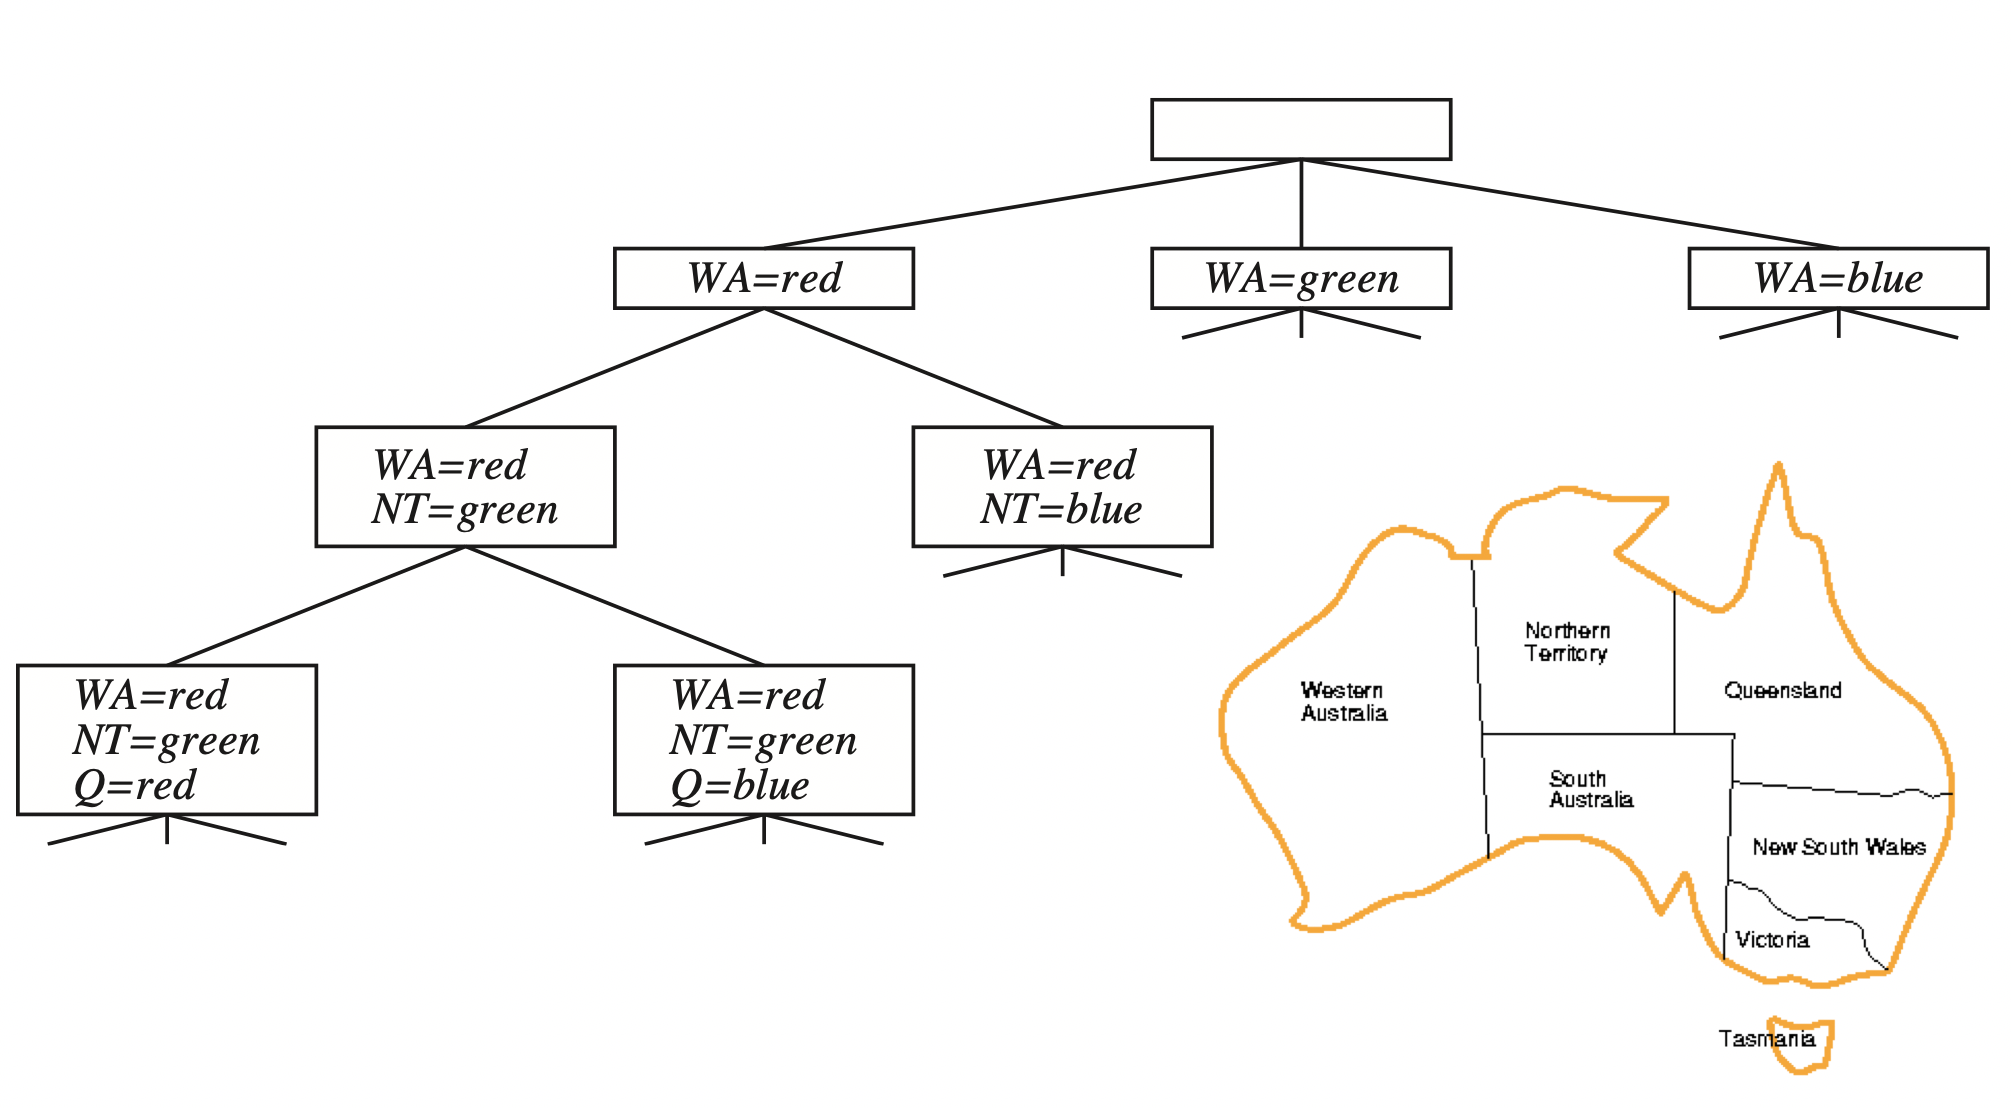
\includegraphics[scale=0.4]{Images/mappacoloratabacktracking.png}
\caption{Problema colorazione mappa con backtracking}
\end{figure}
\clearpage
\subsection{Codice Algoritmo backtracking}
\begin{figure}[h!]
\centering
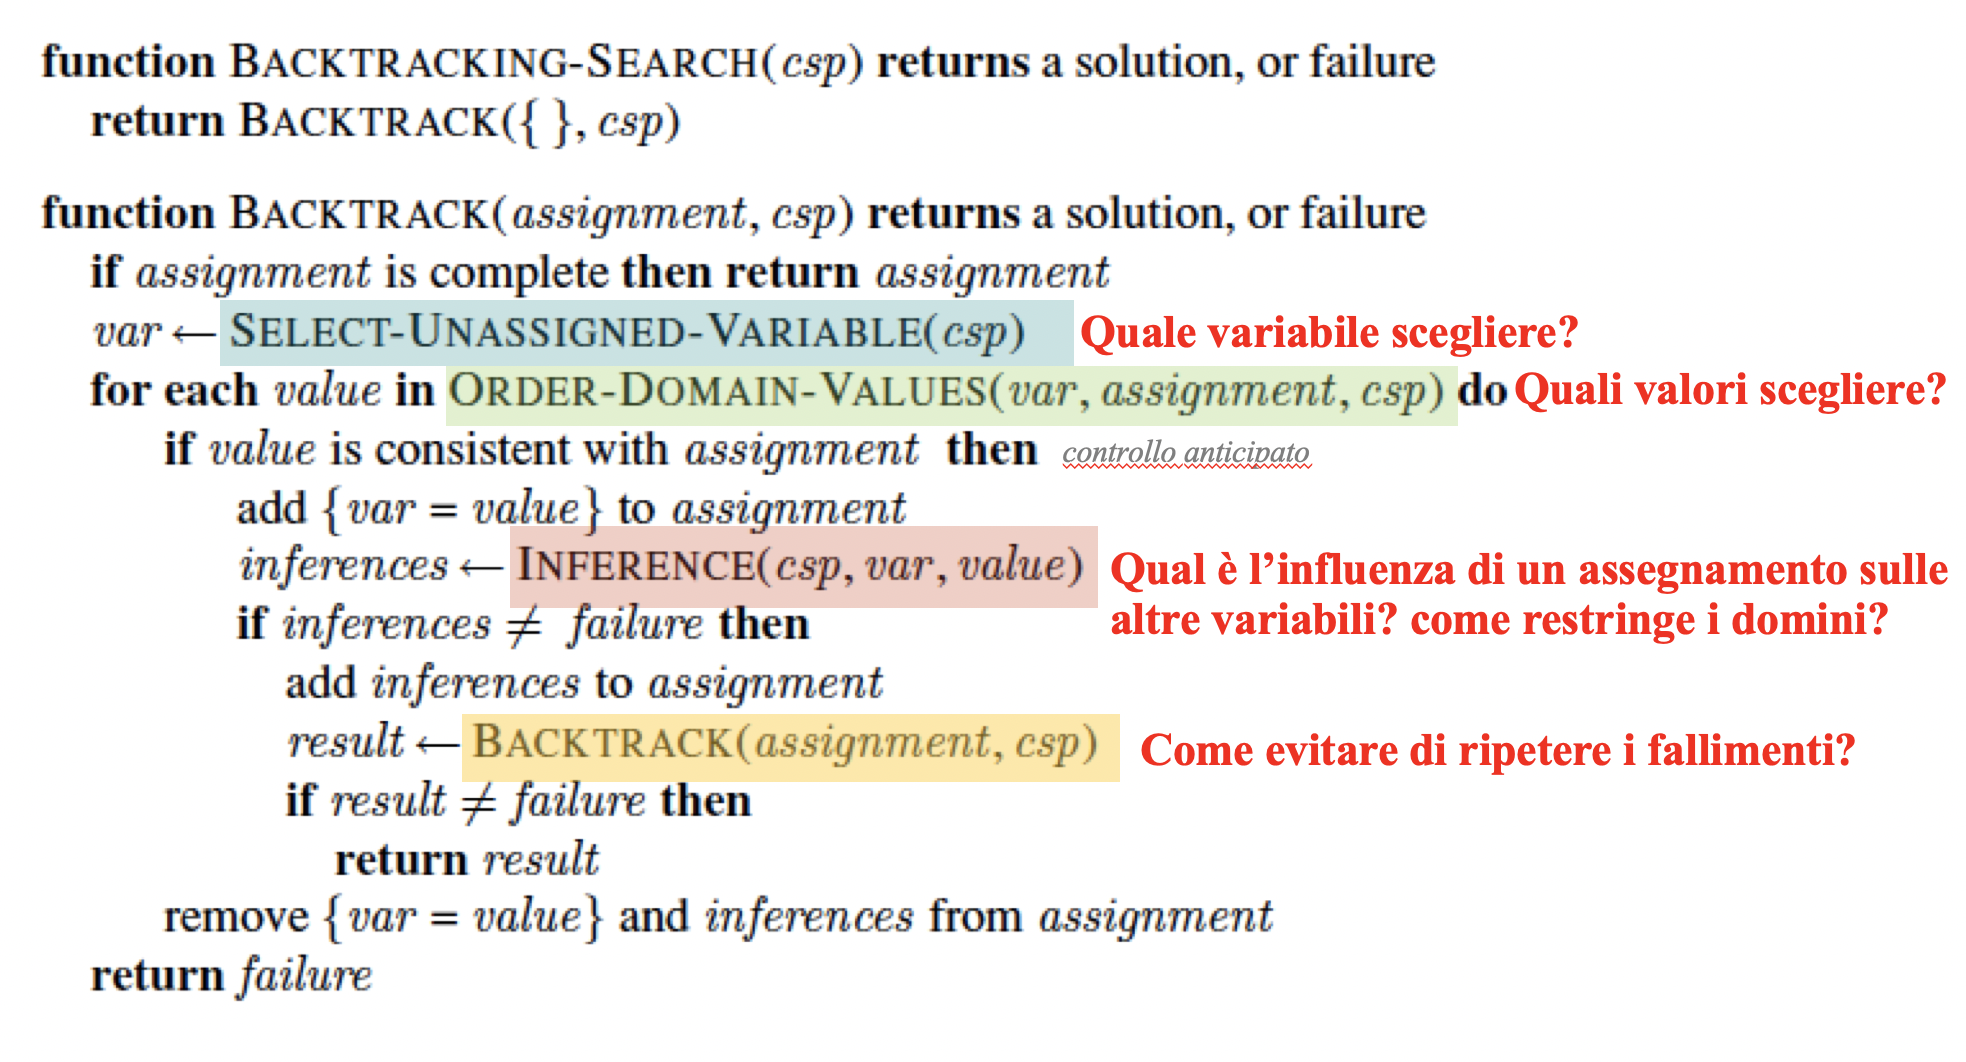
\includegraphics[scale=0.4]{Images/algoritmobacktracking.png}
\end{figure}
le parti evidenziate sono i punti dove posso usare euristiche!
\subsubsection{Select-Unassigned-Variable}
Scelta delle variabili
\begin{itemize}
    \item MRV (Minimum Remaining Values): scegliere la variabile che ha meno valori legali (residui) cioè la variabile più vincolata. Si scoprono prima i fallimenti (fail first)!
    \item Euristica del grado: scegliere la variabile coinvolta in più vincoli con le altre variabili (la variabile più vincolante o di grado maggiore). Da usare a parità di MRV!
\end{itemize}

\subsubsection{Order-Domain-Values}
Scelta dei valori: una volta scelta la variabile come scegliere il valore da assegnare?
\begin{itemize}
    \item Valore meno vincolante: quello che esclude meno valori per le altre variabili direttamente collegate con la variabile scelta. Meglio valutare prima un assegnamento che ha più probabilità di successo, se volessimo tutte le soluzioni l’ordine non sarebbe importante.
\end{itemize}

\subsubsection{Inference}
Propagazione di vincoli, influenza di un assegnamento sulle altre variabili.
\begin{itemize}
    \item Verifica in avanti (Forward Checking o FC): assegnato un valore ad una variabile si possono eliminare i valori incompatibili per le altre variabili direttamente collegate da vincoli
    \item Consistenza di nodo e d’arco: si restringono il valori dei domini delle variabili tenendo conto dei vincoli unari e binari su tutto il grafo (si itera finché tutti i nodi ed archi sono consistenti)
\end{itemize}

\subsubsection{Backtrack}
Si considerano alternative solo per le variabili che hanno causato il fallimento ($X_i, X_j ...$), l’insieme dei conflitti. \\
Ad esempio nelle regine si parte con tutte le variabili assegnate (tette le regine sulla scacchiera), ad ogni passo si modifica l’assegnamento ad una variabile per cui un vincolo è violato (si muove una regina minacciata su una colonna).
È un algoritmo di riparazione euristica: un’euristica potrebbe anche essere scegliere un nuovo valore che crea meno conflitti.

\section{Agenti KB}
Vogliamo adesso migliorare le capacità razionali dei nostri agenti dotandoli di rappresentazioni di mondi più complessi, non descrivibili in modo semplice. Agenti basati su conoscenza, dotati di una KB (knowledge base) con conoscenza espressa in maniera esplicita e dichiarativa.
Ci serve una rappresentazione parziale e incompleta (una astrazione) del mondo, utile agli scopi dell’agente. Per ambienti parzialmente osservabili e complessi ci servono linguaggi di rappresentazione della conoscenza più espressivi e con capacità inferenziali. La conoscenza può essere codificata a mano ma anche estratta dai testi o appresa dall’esperienza.
\subsection{Approccio dichiarativo VS Approccio procedurale}
L'approccio dichiarativo consiste nella creazione di una KB che racchiude tutta la conoscenza necessaria a decidere l’azione da compiere in forma dichiarativa. L’alternativa (approccio procedurale) è scrivere un programma che implementa il processo decisionale, una volta per tutte.
Un agente KB è più flessibile: più semplice acquisire conoscenza incrementalmente e modificare il comportamento con l’esperienza! 
Ricapitolando: un agente basato su conoscenza mantiene una base di conoscenza (KB), cioè un insieme di enunciati espressi in un linguaggio di rappresentazione. L'agente interagisce con la KB mediante una interfaccia funzionale definita come Tell-Ask:
\begin{itemize}
    \item Tell: per aggiungere nuovi enunciati a KB
    \item Ask: per interrogare la KB
    \item Retract: per eliminare enunciati
\end{itemize}
Gli enunciati nella KB rappresentano le credenze dell’agente, le risposte X dell'agente quindi devono essere tali che X è una conseguenza (discende necessariamente) della KB. 
\subsection{Base di conoscenza o Base di dati?}
\begin{itemize}
    \item Base di conoscenza: una rappresentazione esplicita, parziale e compatta, in un linguaggio simbolico, che contiene: fatti di tipo specifico e fatti di tipo generale o regole. Quello che caratterizza una Base di conoscenza è la capacità inferenziale cioè la capacità di derivare nuovi fatti da quelli memorizzati esplicitamente. 
    \item Base di dati: solo fatti specifici e posso solo interrogarla
\end{itemize}
Ma il problema fondamentale della rappresentazione della conoscenza sta nel trovare il giusto compromesso tra: espressività del linguaggio di rappresentazione e complessità del meccanismo inferenziale. Sfortunatamente più il linguaggio è espressivo, meno  efficiente è il meccanismo inferenziale. 

\subsection{Formalismi per la rappresentazione della conoscenza}
Un formalismo per la rappresentazione della conoscenza ha tre componenti:
\begin{enumerate}
    \item Una sintassi: cioè un linguaggio composto da un vocabolario e regole per la formazione delle frasi (enunciati)
    \item Una semantica: che stabilisce una corrispondenza tra gli enunciati e fatti del mondo. Se un agente ha un enunciato X nella sua KB, crede che il fatto corrispondente sia vero nel mondo
    \item Un meccanismo inferenziale: (codificato o meno tramite regole di inferenza come nella logica) che ci consente di inferire nuovi fatti. 
\end{enumerate}
A questo punto, qual è la complessità computazionale del problema KB $\models \alpha$ nei vari linguaggi logici? Quali sono gli algoritmi di decisione e le strategie di ottimizzazione? I linguaggi logici, calcolo proposizionale (PROP) e logica dei predicati (FOL), sono adatti per la rappresentazione della conoscenza?
\section{Agenti Logici: Cacolo proposizionale}
\subsection{Sintassi (regole)}
La sintassi definisce quali sono le frasi legittime (ben formate) del linguaggio.
\begin{itemize}
    \item simbolo $\to$ P | Q | S ...
    \item formula $\to$ formulaAtomica | formulaComplessa
    \item formulaAtomica $\to$ Ture | False | simbolo
    \item formulaComplessa $\to \neg$ formula | formula $\land$ formula | formula $\lor$ formula | formula $\Rightarrow$ formula | formula $\Leftrightarrow$ formula
\end{itemize}
Possiamo omettere le parentesi assumendo questa precedenza tra gli operatori:
\begin{quote}
    $\neg  >  \land  >  \lor  >  \Rightarrow, \Leftrightarrow$
\end{quote}

\subsection{Semantica (significato)}
La sematica definisce se un enunciato è vero o falso rispetto ad una interpretazione. Una interpretazione definisce un valore di verità per tutti i simboli proposizionali. Il significato di una frase è determinato dal significato dei suoi componenti, a partire dalle frasi atomiche (i simboli proposizionali). 

\subsection{Conseguenza logica}
Il problema: data una base di conoscenza KB, contenente una rappresentazione dei fatti che si ritengono veri, vorrei sapere se un certo fatto $alpha$ è vero di conseguenza cioè se KB $\models \alpha$ (conseguenza logica).
Una formula $\alpha$ è conseguenza logica di un insieme di formule KB se e solo se in ogni modello di KB $\alpha$ è vera (KB $\models \alpha$). \newline Indicando con M($\alpha$) i modelli di $\alpha$ cioè l’insieme delle interpretazioni che rendono $\alpha$ vera, e con M(KB) i modelli dell’insieme di formule in KB otteniamo:
\begin{quote}
    KB $\models \alpha \Leftrightarrow$ M(KB) $\subseteq$ M($\alpha$)
\end{quote}

\subsection{Il mondo del Wumpus}
Il mondo del Wumpus è una caverna fatta di stanze connesse tra di loro attraverso passaggi. Il Wumpus mangia chiunque entri nella stanza in cui si trova. Il wumpus può essere ucciso dall’agente, che ha solo una freccia a disposizione. Ci sono stanze con dei pozzi: se l’agente entra in una di queste stanze cade nel pozzo e muore. In una delle stanze si trova l’oro e l’obiettivo dell’agente è di trovarlo l’oro e tornare a casa sano e salvo. L’agente non conosce l’ambiente, né la sua locazione. Solo all’inizio sa dove si trova (in [1,1]).
Gli ambienti sono generati a caso e alcuni di questi non sono risolubili (ma sappiamo che lo stato (1,1) è safe): l’agente in alcune situazioni deve decidere se rischiare di essere ucciso pur di trovare l’oro e quando conviene tornare a casa a mani vuote.
\begin{figure}[h!]
\centering
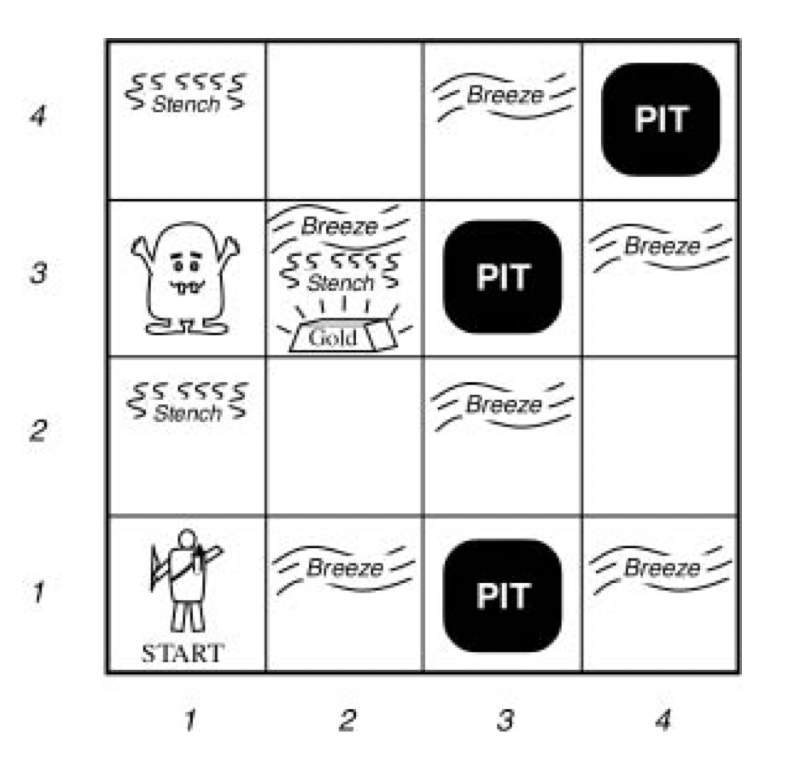
\includegraphics[scale=0.5]{Images/wumpus_a.png}
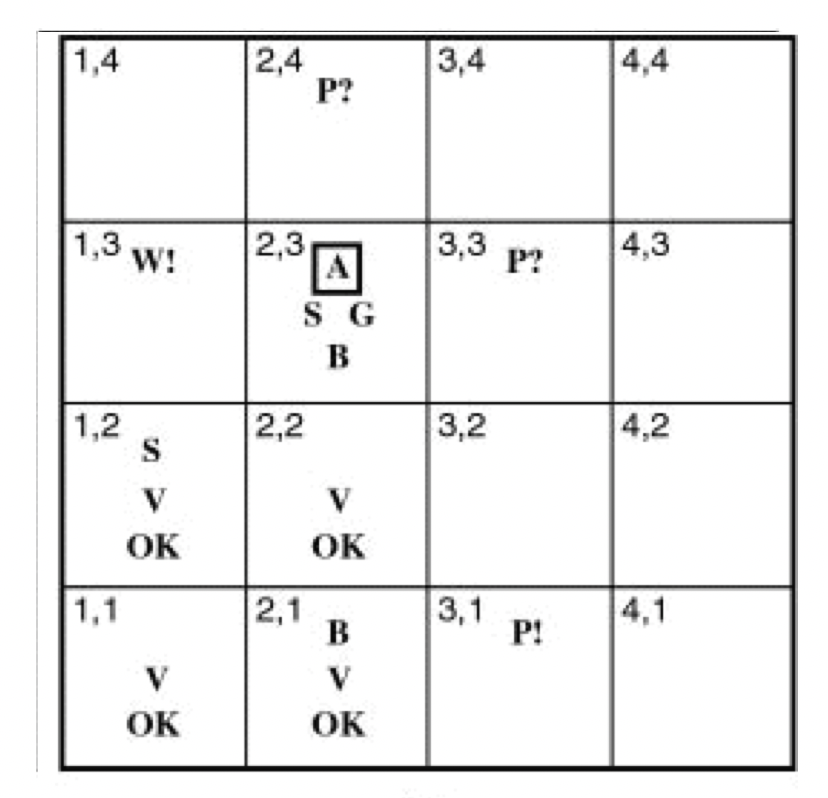
\includegraphics[scale=0.5]{Images/wumpus_b.png}
\caption{Wumpus' world}
\end{figure}
\begin{itemize}
    \item Misura delle prestazioni:
    \begin{itemize}
        \item +1000 se trova l’oro, torna in [1,1] e esce
        \item -1000 se muore
        \item -1 per ogni azione
        \item -10 se usa la freccia
    \end{itemize}
    \item Percezioni:
    \begin{itemize}
        \item \textbf{puzzo} nelle caselle adiacenti al Wumpus
        \item \textbf{brezza} nelle caselle adiacenti alle buche
        \item \textbf{luccichio} nelle caselle con l‘oro
        \item \textbf{bump } se sbatte in un muro
        \item \textbf{urlo} se il Wumpus viene ucciso
        \item L’agente non percepisce la sua locazione
    \end{itemize}
    \item Azioni:
    \begin{itemize}
        \item avanti
        \item destra
        \item sinistra
        \item afferra oggetto
        \item scaglia la freccia
        \item esci
    \end{itemize}
\end{itemize}
Le percezioni sono una quintupla [puzzo, brezza, luccichio, bump, urlo]. ([none, none, none, none, none] se non percepisce niente).
\subsubsection{Esempio dal mondo del Wumpus}
KB = $B_{2,1}, \neg B_{1,1} , +$ le regole del WumpusWorld \newline 
Vogliamo stabilire l’assenza di pozzi in [1,2] e in [2,2] \newline
KB $\models \neg P_{1,2}$? \newline
KB $\models \neg P_{2,2}$? \newline
Ci sono otto possibili interpretazioni o mondi, considerando solo l’esistenza di pozzi nelle 3 caselle $P_{1,2} \quad P_{2,2} \quad P_{3,1}$ a sinsitra prendiamo tutti i mondi in cui non c'è pozzo in [1,2] e includo tutti i mondi compatibili con la mia KB, a destra quelli dove non c'è pozzo in [2,2] e vediamo che questi non includono tutti i mondi nella mia KB quindi KB $\nvDash \neg P_{2,2}$ .
\begin{figure}[h!]
\centering
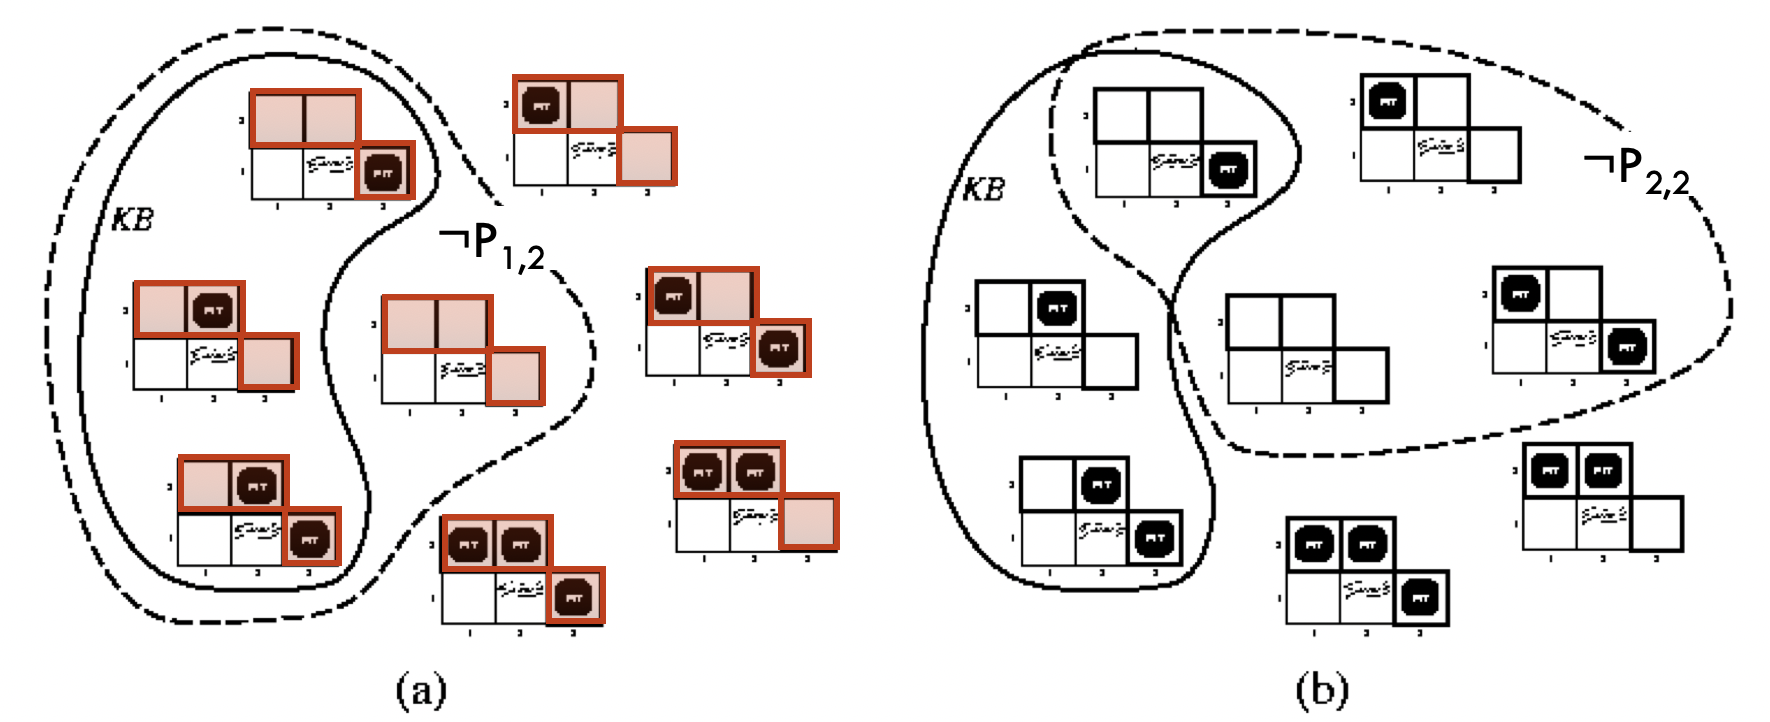
\includegraphics[scale=0.45]{Images/wumpusconslogica.png}
\end{figure}
\subsection{Formule logiche, Validità e Soddisfacibilità}
\begin{figure}[h!]
\centering
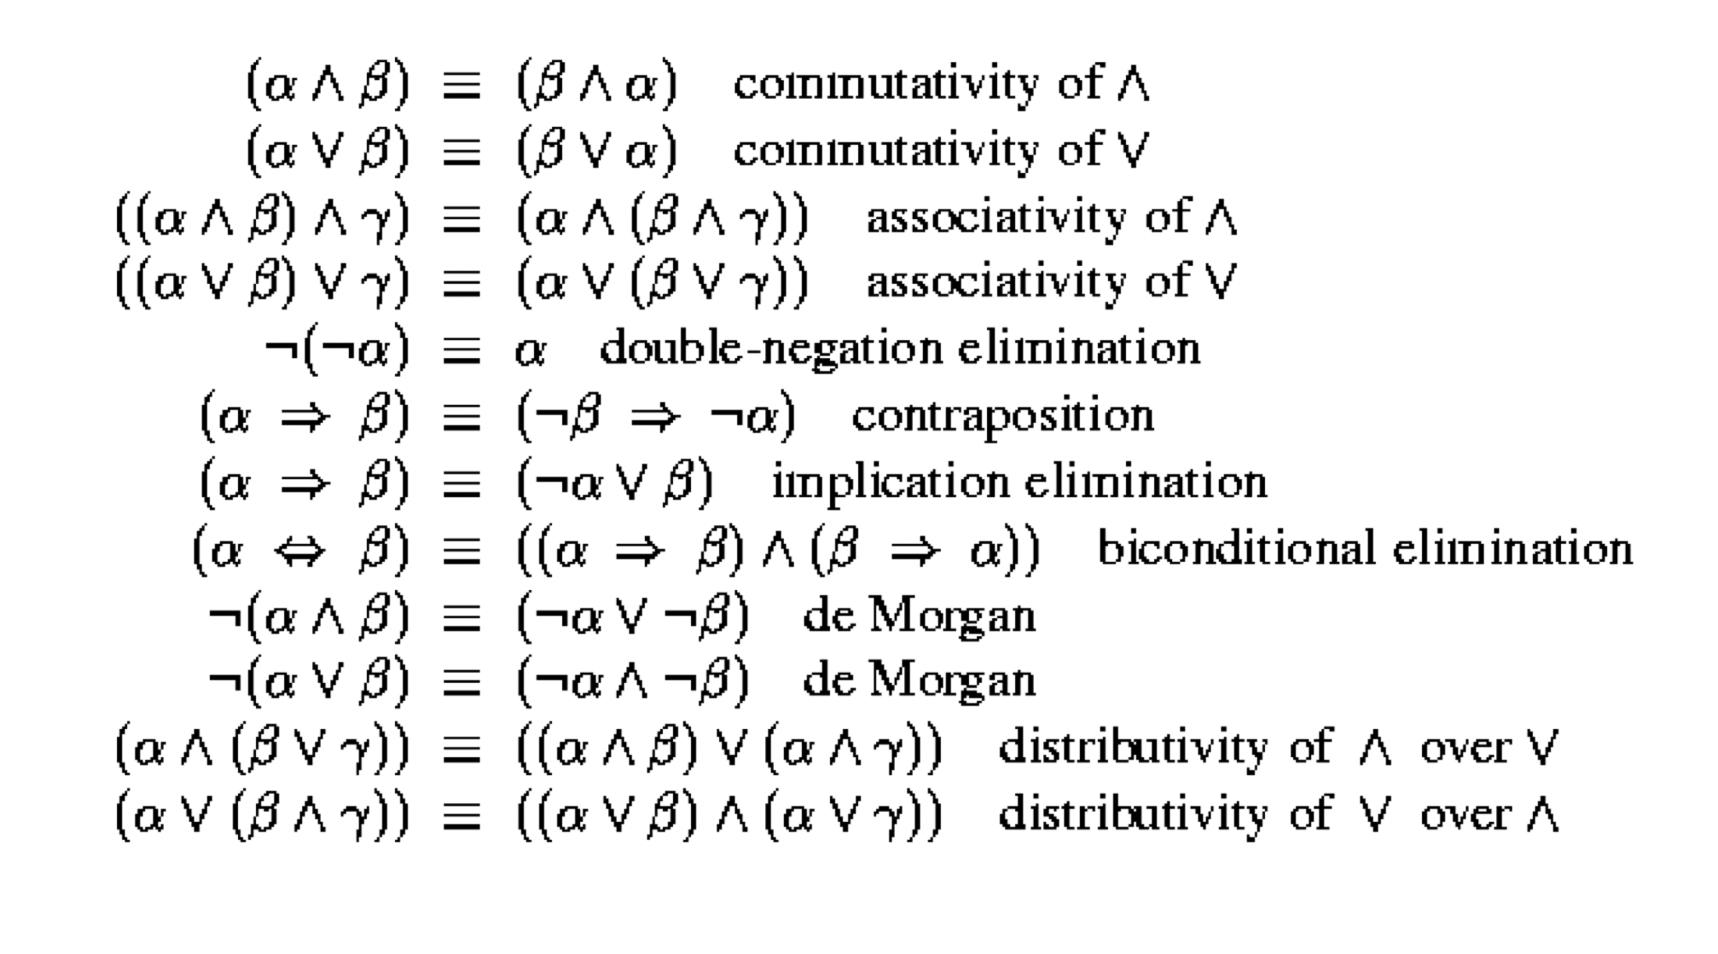
\includegraphics[scale=0.35]{Images/formulelogiche.png}
\end{figure}
A valida sse è vera in tutte le interpretazioni (anche detta tautologia). \newline
A soddisfacibile sse esiste una interpretazione in cui A è vera. \newline
A è valida sse $\neg$A è insoddisfacibile. \newline
\subsection{Inferenza per calcolo proposizionale}
\begin{itemize}
    \item Model checking: una forma di inferenza che fa riferimento alla definizione di conseguenza logica (si enumerano i possibili modelli e si controllano tramite le tabelle di verità)
    \item Algoritmi per la soddisfacibilità: problemi riconducibili ad altri problemi. \newline KB $\models$ A sse $KB\land \neg A$ è insoddisfacibile.
\end{itemize}
\subsection{Algoritmo TT-Entails (Model Checking)}
Come facciamo a sapere se KB $\models \alpha$? L'algoritmo TT-Entails enumera tutte le possibili interpretazioni di KB (k simboli, $2^k$ possibili interpretazioni). Per ciascuna interpretazione 
\begin{itemize}
    \item Se non soddisfa KB $\to$ OK (se alla fine tutti OK è conseguenza logica)
    \item Se soddisfa KB, si controlla che soddisfi anche $\alpha$. Se si trova anche solo una interpretazione che soddisfa KB e non $\alpha$ la risposta è NO.
\end{itemize} 
\subsubsection{Esempio TT-Entails}
\begin{figure}[h!]
\centering
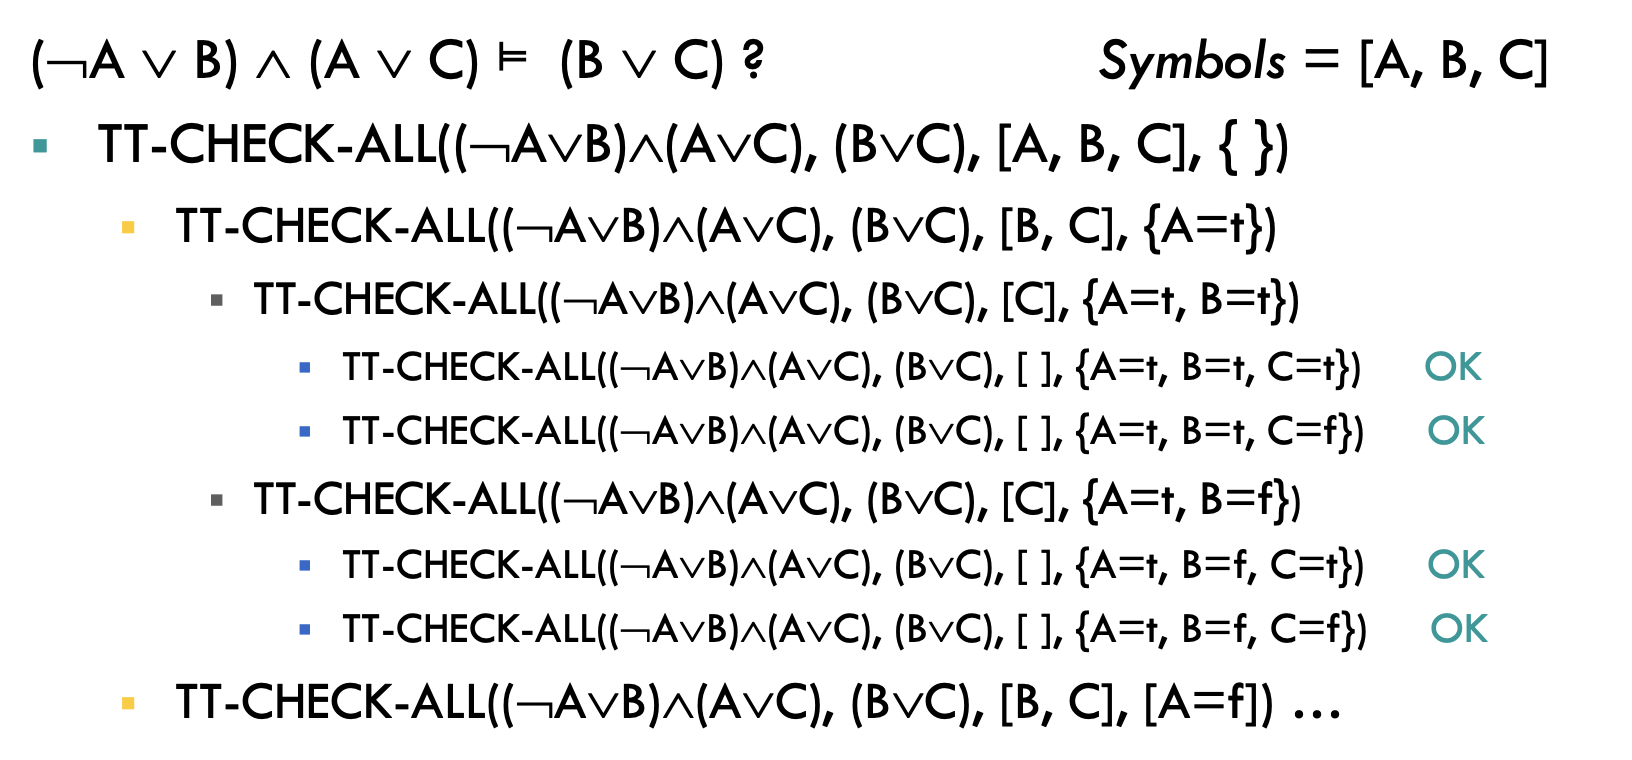
\includegraphics[scale=0.4]{Images/ttentailscheck.png}
\end{figure}
Solo alla fine, dopo avere provato tutti i possibili assegnamenti, possiamo rispondere se Vero o Falso.

\subsection{Algoritmo DPLL (Alg. Soddisfacibilità)}
\subsubsection{Forma a clausole}
Gli algoritmi per la soddisfacibilità usano KB in forma a clausole. \newline 
Esempio: \{A, B\} \{$\neg$B, C, D\} \{$\neg$A, F\} \newline
è una forma normale congiuntiva cioè una congiunzione di disgiunzioni letterali. Il suo significato quindi è: \newline (A $\lor$ B) $\land$ ($\neg$ B $\lor$ C $\lor$ D) $\land$ ($\neg$ A $\lor$ F), la cosa interessante è che non è restrittiva: è sempre possibile ottenerla con trasformazioni che preservano l’equivalenza logica! I passi da seguire sono: \begin{enumerate}
    \item Eliminazione della $\Leftrightarrow$: (A $\Leftrightarrow$ B) $\equiv$ (A $\Rightarrow$ B) $\land$ (B $\Rightarrow$ A)
    \item Eliminazione dell’ $\Rightarrow: (A \Rightarrow B) \equiv (\neg A \lor B)$
    \item Negazioni all’interno: \begin{itemize}
        \item $\neg (A \lor B) \equiv (\neg A \land \neg B)$	(de Morgan)	
        \item $\neg (A \land B) \equiv (\neg A \lor \neg B)$
    \end{itemize}   
    \item Distribuzione di $\lor$ su $\land$: $(A \lor (B \land C)) \equiv (A \lor B) \land (A \lor C)$
\end{enumerate}
L'algoritmo DPLL sfrutta la soddisfacibilità di $KB \models A$ se $KB \land \neg A$ = \{\}). Parte da una KB in forma a clausole, avviene una enumerazione in profondità di tutte le possibili interpretazioni alla ricerca di un modello. Tre miglioramenti rispetto a TTEntails: 
\begin{enumerate}
    \item Terminazione anticipata: Si può decidere sulla verità di una clausola anche con interpretazioni parziali: basta che un letterale sia vero. Ad esempio se A è vero lo sono anche \{A, B\} e \{A, C\} indipendentemente dai valori di B e C. (ricordiamo che sono in $\lor$!). Se anche una sola clausola è falsa l'interpretazione non può essere un modello dell’insieme di clausole. 
    \item Simboli puri: un simbolo puro è un simbolo che appare con lo stesso segno in tutte le clausole. Ad esempio \{A, $\neg B\} \{ \neg B, \neg C\} \{C, A\}$ dove A e B sono puri. Nel determinare se un simbolo è puro se ne possono trascurare le occorrenze in clausole già rese vere cioè i simboli puri possono essere assegnati a True se il letterale è positivo, False se negativo. Facendo così non si eliminano modelli utili: se le clausole hanno un modello continuano ad averlo dopo questo assegnamento. L’assegnamento è obbligato.
    \item Clausole unitarie: una clausola con un solo letterale non assegnato, ad esempio \{B\} è unitaria ma anche \{B, $\neg$C\} è unitaria quando C = True. Conviene assegnare prima valori al letterale in clausole unitarie. L'assegnamento è univoco (True se positivo, False se negativo).
\end{enumerate}
\subsubsection{Esempio DPLL}
KB $\{\neg B_{1,1}, P_{1,2}, P_{2,1}\} \{\neg P_{1,2}, B_{1,1}\} \{\neg P_{2,1}, B_{1,1}\} \{\neg B_{1,1}\} \models \{\neg P_{1,2} \}$? \newline
Aggiungiamo \{$P_{1,2}$\} (perchè sarebbe $\neg (\neg P_{1,2})$ e vediamo se l’insieme è insoddisfacibile: \newline 
SAT($\{\neg B_{1,1}, P_{1,2}, P_{2,1}\} \{\neg P_{1,2}, B_{1,1}\} \{\neg P_{2,1}, B_{1,1}\} \{\neg B_{1,1}\} \{P_{1,2} \}$) \newline
Notiamo che \{$P_{1,2}$ \} è unitaria quindi assegnamo $P_{1,2}$=True. \newline
La prima clausola $\{\neg B_{1,1}, P_{1,2}, P_{2,1}\}$ e  $\{P_{1,2} \}$ sono soddisfatte. \newline
La seconda clausola $\{\neg P_{1,2}, B_{1,1}\}$ diventa unitaria, $B_{1,1}$=True. A questo punto $\{\neg P_{1,2}, B_{1,1}\}$ e $\{\neg P_{2,1}, B_{1,1}\}$ sono soddisfatte, ma $\{\neg B_{1,1}\}$ no. FAIL! \newline Non esistono modelli, quindi $\neg P_{1,2}$ è conseguenza logica della KB.
\subsubsection{Miglioramenti DPLL}
DPLL è completo e termina sempre. Alcuni miglioramenti: Analisi di componenti (se le variabili possono essere suddivise in sotto-insiemi disgiunti (senza simboli in comune)), Ordinamento di variabili e valori (scegliere la variabile che compare in più clausole), Backtracking intelligente e altre ottimizzazioni...
\subsection{Algoritmo WALK-SAT}
Gli stati sono assegnamenti completi, l’obiettivo è un assegnamento che soddisfa tutte le clausole (un modello) partendo da un assegnamento casuale. Ad ogni passo si cambia il valore di una proposizione (flip). Gli stati sono valutati contando il numero di clausole non soddisfatte [o soddisfatte] (meno sono meglio è). Ci sono molti minimi locali, per non incapparci serve introdurre perturbazioni casuali, come Hill climbing con riavvio casuale o Simulated Annealing. WALK-SAT è uno degli algoritmi più semplici ed efficaci. \newline 
WalkSAT ad ogni passo: 
\begin{itemize}
    \item Sceglie a caso una clausola non ancora soddisfatta
    \item Sceglie un simbolo da modificare (flip) scegliendo con probabilità p (di solito 0,5) tra una delle due: \begin{itemize}
        \item Passo casuale: un simbolo a caso
        \item Passo di ottimizzazione: sceglie quello che rende più clausole soddisfatte
    \end{itemize}
    \item Si arrende dopo un certo numero di flip predefinito (variabile max-flips)
\end{itemize}
\subsubsection{Esempio WALK-SAT}
Come euristica usiamo il numero di clausole soddisfatte (valore da massimizzare). \newline
\textcolor{red}{Rosso: passo casuale} \newline
\textcolor{blue}{Blu: passo di ottimizzazione} \newline
$(1)\{\neg B_{1,1}, P_{1,2}, P_{2,1}\} (2)\{\neg P_{1,2}, B_{1,1}\} (3)\{\neg P_{2,1}, B_{1,1}\} (4)\{\neg B_{1,1}\}$ \newline
[$B_{1,1}=F, P_{1,2}=T, P_{2,1}=T$] \textcolor{red}{clausole 2, 3 F; scelgo clausola 2; a caso eseguo flip $B_{1,1}$} \newline
[$B_{1,1}=T, P_{1,2}=T, P_{2,1}=T$] \textcolor{blue}{clausola 4 F; scelgo 4; ottimizzazione: flip $B_{1,1}$ (unica scelta)}\newline
[$B_{1,1}=F, P_{1,2}=T, P_{2,1}=T$] \textcolor{red}{clausole 2, 3 F; scelgo clausola 2; a caso eseguo flip $P_{1,2}$}\newline
[$B_{1,1}=F, P_{1,2}=F, P_{2,1}=T$] \textcolor{blue}{clausola 3 F; scelgo 3; ottimizzazione: flip $P_{2,1}$}\newline
[$B_{1,1}=F, P_{1,2}=F, P_{2,1}=F$]   modello\newline
\subsection{Analisi WALK-SAT}
Se max-flips = $\infty$ e l’insieme di clausole è soddisfacibile prima o poi termina. Va bene per cercare un modello, sapendo che esiste, ma se è insoddisfacibile non termina. Non può essere usato per verificare l’insoddisfacibilità, il problema quindi è decidibile ma l’algoritmo non è completo. \newline
\subsubsection{Problemi SAT difficili}
Se un problema ha molte soluzioni (problema sotto-vincolato) è più probabile che WALK-SAT ne trovi una in tempi brevi. Ad esempio: esistono 16 soluzioni su 32 assegnamenti possibili, un assegnamento ha il 50\% di probabilità di essere giusto: 2 passi in media!
Un altro esempio che si può fare è che in questa istanza: \newline $(\neg D \lor \neg B \lor C) \land (B \lor \neg A \lor \neg C) \land (\neg C \lor \neg B \lor E) \land (E \lor \neg D \lor B) \land (B \lor E \lor \neg C)$ \newline quello che conta è il rapporto m/n, dove m è il numero di clausole (vincoli) e n il numero di simboli. In questo esempio 5/5=1, più è grande il rapporto, più vincolato è il problema.
\begin{figure}[h!]
\centering
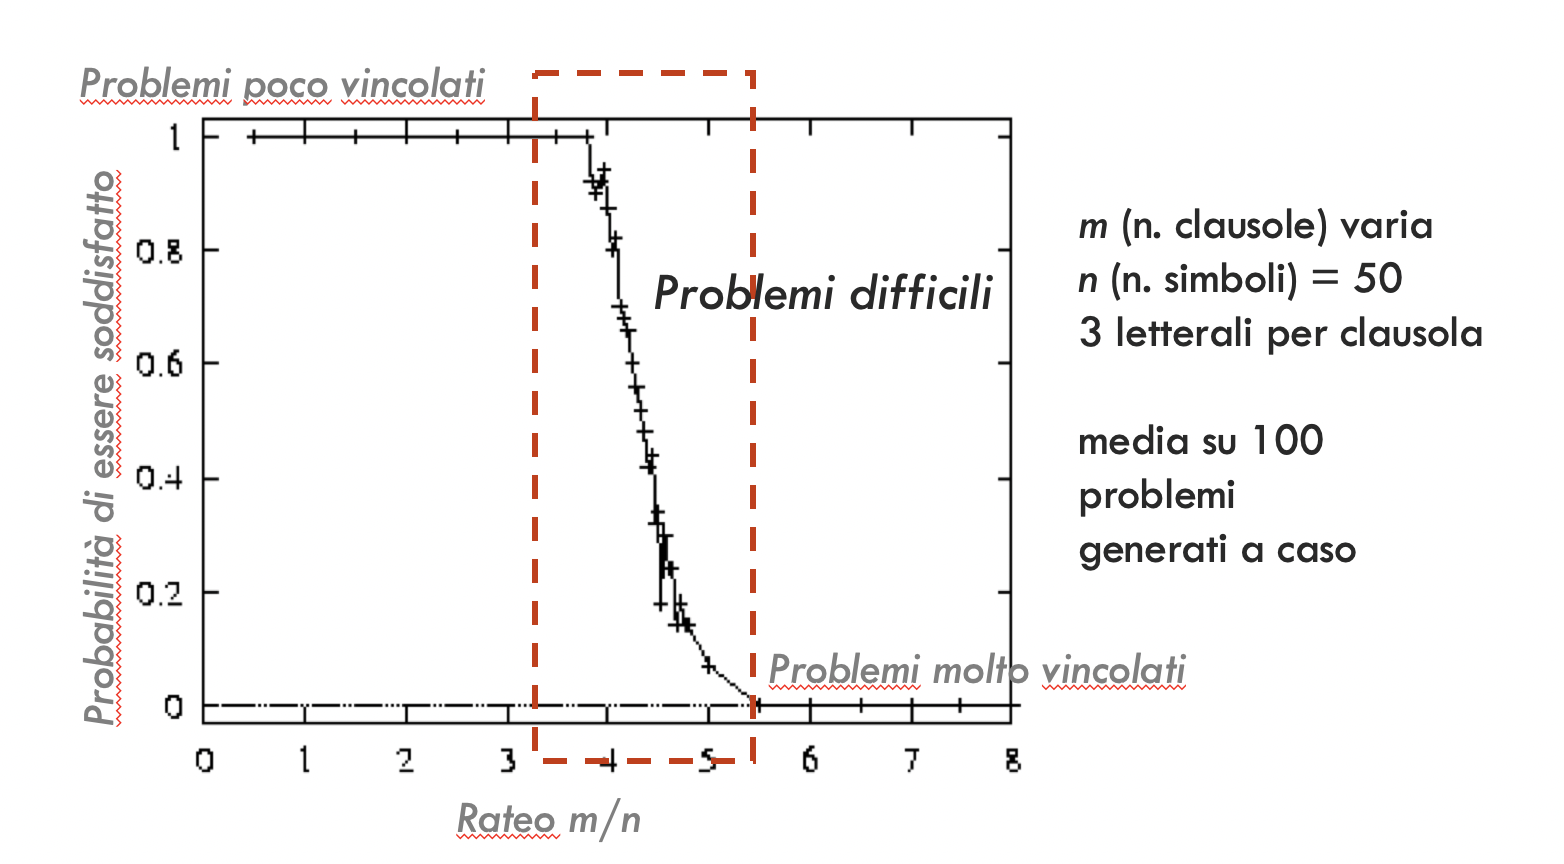
\includegraphics[scale=0.35]{Images/rateomn.png}
\end{figure}
\subsection{Inferenza come deduzione}
Un altro modo per decidere se KB $\models$ A è usare un meccanismo di dimostrazione (deduzione). Si scrive KB $\vdash$ A  (A è deducibile da KB). La deduzione avviene specificando delle regole di inferenza.
\begin{itemize}
    \item Correttezza: Se KB $\vdash$ A allora KB $\models$ A. Tutto ciò che è derivabile è conseguenza logica.
    \item Completezza: Se KB $\models$ A allora KB $\vdash$ A. Tutto ciò che è conseguenza logica è ottenibile tramite il meccanismo di inferenza.
\end{itemize}
Nota: questa nozione di completezza (detta anche completezza semantica) si riferisce al teorema di completezza di Godel. Il teorema di incompletezza di Godel non asserisce che non esistono sistemi deduttivi completi per il FOL, ma che una logica abbastanza potente da assiomatizzare l’aritmetica non è in grado di dimostrare tutte le asserzioni vere sui numeri.
\subsubsection{Alcune regole di inferenza}
Modus Ponens \quad
\infer{\beta}{
    \alpha \rightarrow \beta
    & \deduce{\alpha}
} \newline
Eliminazione dell'AND \quad
\infer{\alpha}{
    \alpha \land \beta
} \newline
Eliminazione doppia implicazione \quad
\infer{(\alpha \Rightarrow \beta) \land (\beta \Rightarrow \alpha)}{
    \alpha \Leftrightarrow \beta
} \newline
Introduzione doppia implicazione \quad
\infer{\alpha \Leftrightarrow \beta}{
    (\alpha \Rightarrow \beta) \land (\beta \Rightarrow \alpha)
} \newline

Come decidere ad ogni passo qual è la regola di inferenza da applicare? e a quali premesse applicarla? Nasce quindi un problema di esplorazione di uno spazio di stati. Una procedura di dimostrazione definisce quindi sia la direzione della ricerca che una strategia di ricerca.

\subsubsection{Direzione della ricerca}
Nella dimostrazione di teoremi conviene procedere all’indietro. Se si vuole dimostrare A $\land$ B si cerca di dimostrare A e poi B, se si vuole dimostrare A $\Rightarrow$ B, si assume A e si cerca di dimostrare B.
\subsubsection{Strategia di ricerca}
Completezza: Le regole della deduzione naturale sono un insieme di regole di inferenza completo, se l’algoritmo di ricerca è completo siamo a posto! \newline
Efficienza: La complessità è alta, è un problema decidibile ma NP-completo.
\subsection{Regola di risoluzione}
Un’unica regola: la regola di risoluzione (presuppone forma a clausole). Esempio: \newline
\infer{\{Q,R\}}{
    \{P,Q\}
    & \deduce{\{\neg P,R\}}
} \quad 
\infer{Q \lor R}{
    P \lor Q
    & \deduce{\neg P \lor R}
}
\subsubsection{Regola di risoluzione in generale}
\quad
\infer{\{ I_1,I_2, ..., I_i, ..., I_k \} \{ M_1,M_2, ..., M_j, ..., M_n \}}{
    \{ I_1,I_2, ..., I_{i-1}, I_{i+1} ..., I_k, M_1,M_2, ..., M_{j-1},M_{j+1} ..., M_n \}
} \newline
Gli "I" e "M" sono letterali, simboli di proposizione positivi o negativi, la cosa fondamentale da sapere è che $I_i$ e $M_j$ sono simboli uguali ma di segno opposto.
Un caso particolare avviene quando ci troviamo in questa situazione: \newline
\quad
\infer{\{\} //clausola vuota \rightarrow contraddizione}{
    \{P\}
    & \deduce{\{\neg P\}}
}
\subsubsection{Esempio grafo di risoluzione}
\begin{figure}[h!]
\centering
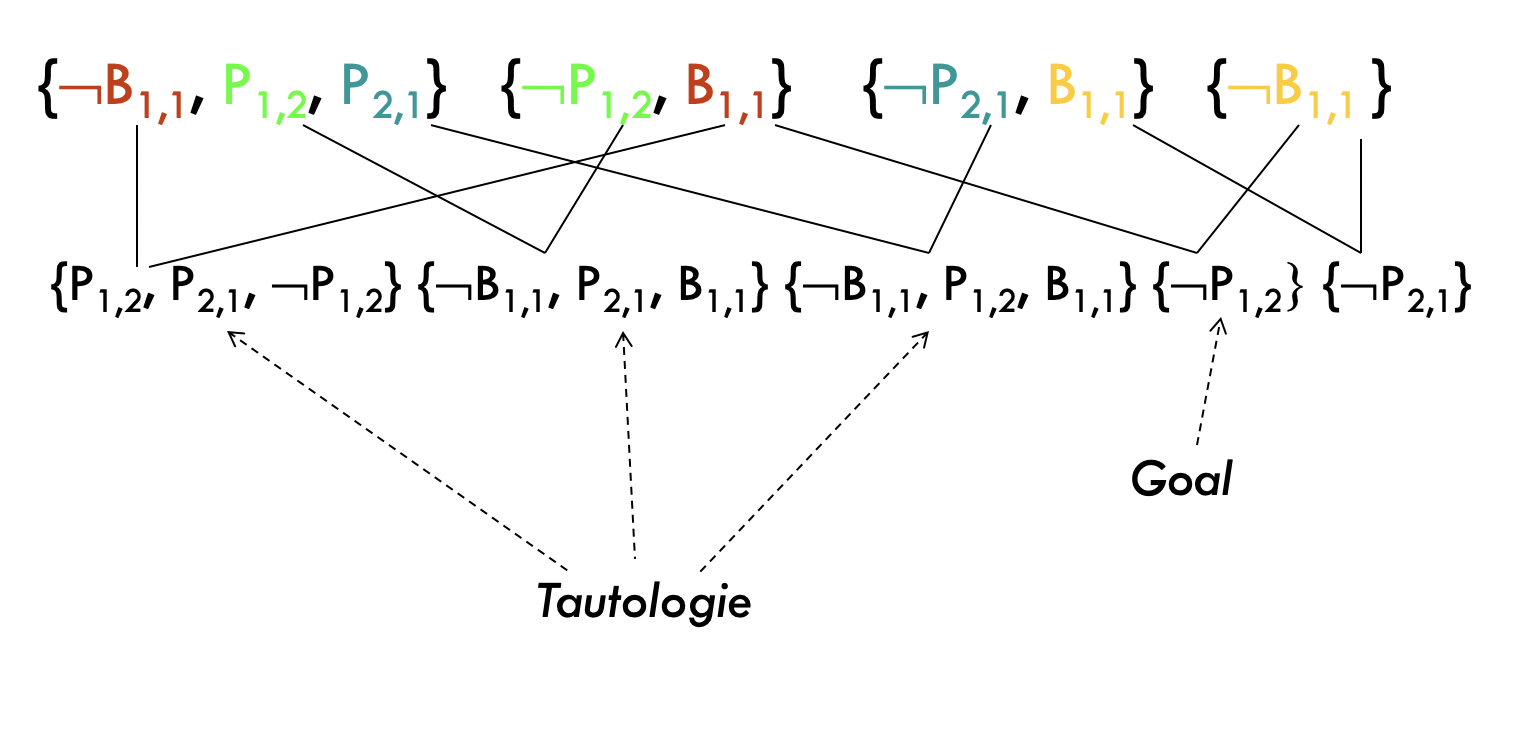
\includegraphics[scale=0.5]{Images/esgraforisoluzione.png}
\end{figure}
ATTENZIONE:
\begin{figure}[h!]
\centering
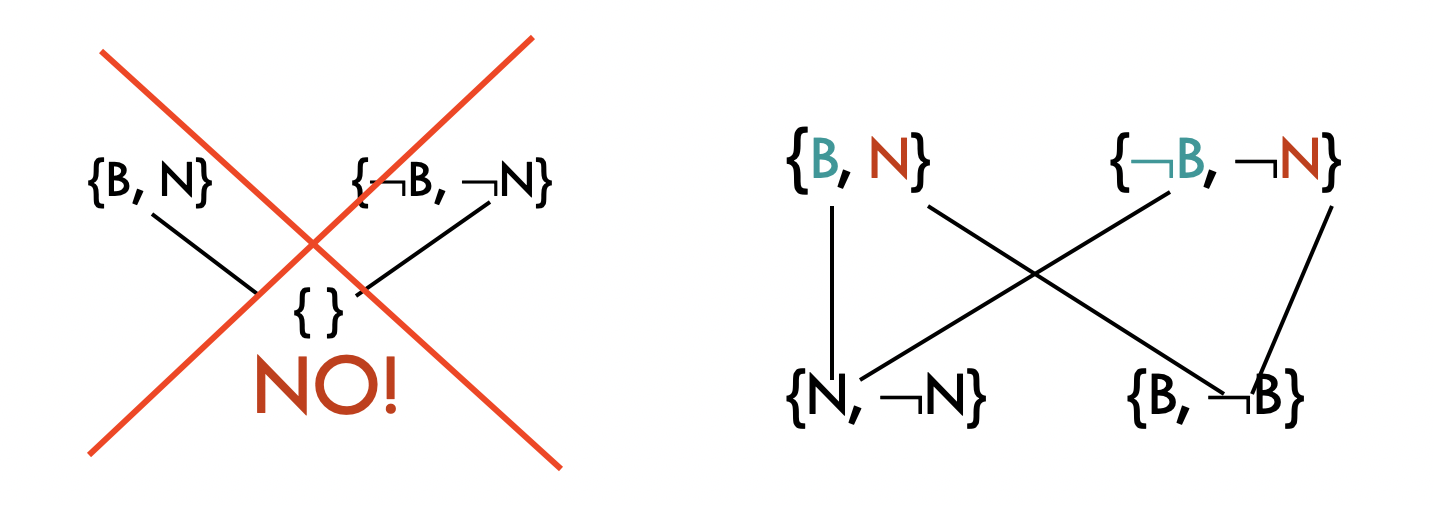
\includegraphics[scale=0.5]{Images/danger.png}
\end{figure}
\subsubsection{Refutazione}
\begin{figure}[h!]
\centering
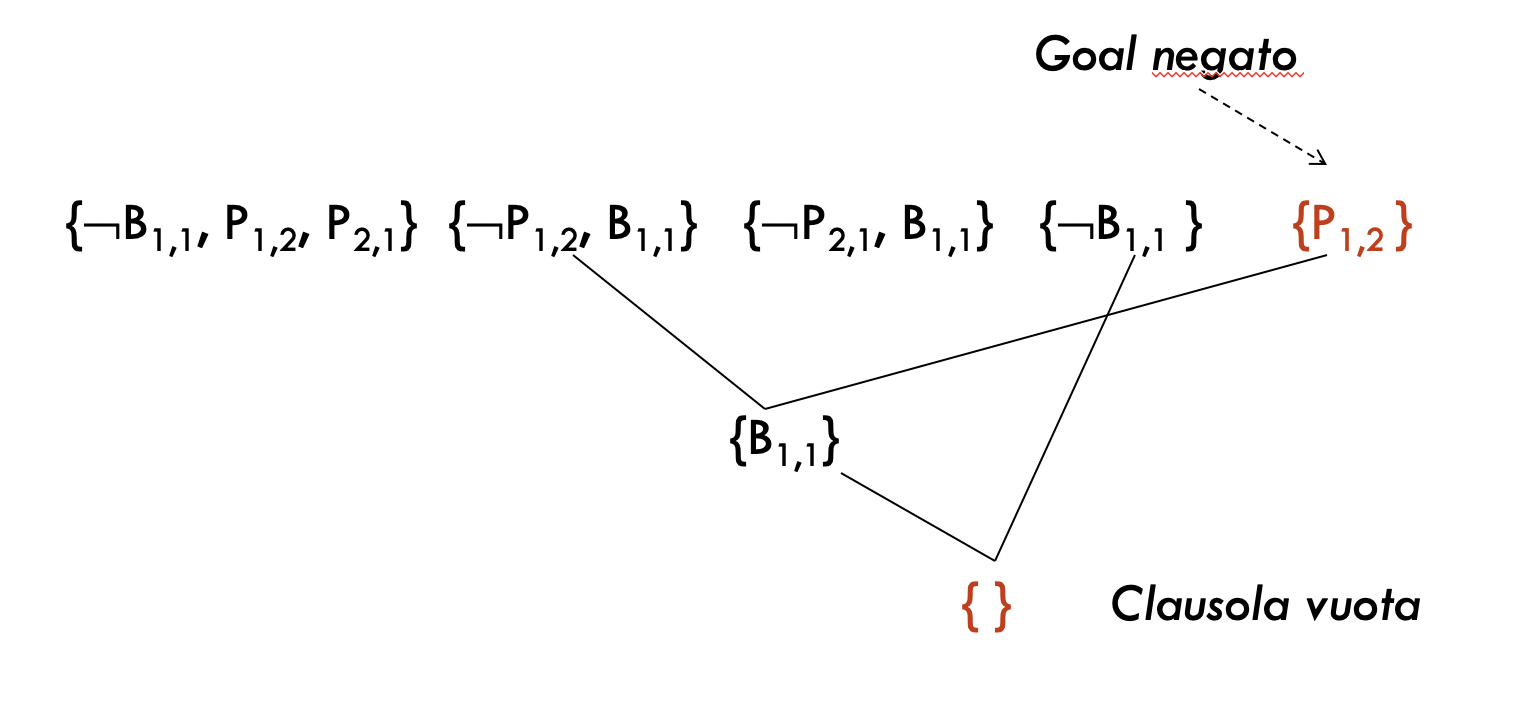
\includegraphics[scale=0.5]{Images/refutazione.png}
\end{figure}
\subsubsection{Osservazioni}
Abbiamo una singola regola di inferenza, ma è sufficiente? Siamo sicuri che applicando la regola in tutti i modi possibili riesco a dedurre A quando è conseguenza logica? Vale la completezza? No. 
Per fortuna il teorema di refutazione ci offre un modo alternativo di procedere: se voglio vedere se A è $\models$ KB, aggiungo $\neg A$ a KB e vedo se l’insieme ottenuto è insoddisfacibile. La correttezza della regola ci dice anche che se da tale insieme derivo la clausola vuota allora in effetti l’insieme è insoddisfacibile. Inoltre abbiano un altro risultato, il teorema di risoluzione, che ci garantisce che se KB è insoddisfacibile allora la clausola vuota sono sempre in grado di trovarla con applicazioni della regola di risoluzione. Concludendo procedere per refutazione ci garantisce la completezza (naturalmente se la procedura applica la regola in maniera sistematica).

\section{Agenti Logici: Logica del prim'ordine}
Nella logica dei predicati abbiamo assunzioni che comprendono gli oggetti, le proprietà e le relazioni. Si inizia con una concettualizzazione, cioè si tratta di decidere quali sono le cose di cui si vuole parlare. 
\begin{itemize}
    \item Gli oggetti: un libro, un evento, una persona... Possono essere identificati con simboli o relativamente ad altri oggetti, mediante funzioni: “la madre di Pietro”. L’insieme degli oggetti rilevanti costituiscono il dominio del discorso. Il dominio potrebbe essere infinito! 
    \item Le proprietà: “la madre di Pietro è simpatica”
    \item Le relazioni tra gli oggetti: “Pietro è amico di Paolo”
\end{itemize} 
\subsubsection{Esempio: il mondo dei blocchi}
\begin{itemize}
    \item Dominio: \{a, b, c, d, e\} (blocchi veri)
    \item Le funzioni: si individuano le funzioni rilevanti che servono anch’esse per identificare oggetti. Ad esempio la funzione "Hat(x)" che dato un blocco "x" identifica il blocco ad esso superiore.
    \item Le relazioni: si individuano le relazioni interessanti. \begin{itemize}
        \item On = $\{<a, b>, <b, c>, <d, e>\}$ //a è su b, b è su c, d è su e
        \item Clear = \{a, d\} //non hanno nulla sopra di loro
        \item Table = \{c, e\} //sono poggiati sul tavolo
        \item Block = \{a, b, c, d, e\} //sono blocchi
    \end{itemize} 
\end{itemize}
\begin{figure}[h!]
\centering
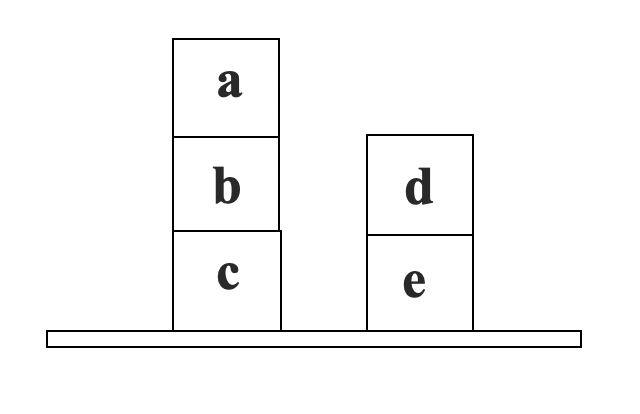
\includegraphics[scale=0.3]{Images/blocks.png}
\end{figure}
\subsubsection{Concettualizzazioni}
Otteniamo così la concettualizzazione del problema definita come \newline $<\{a, b, c, d, e\}, \{Hat\}, \{On, Clear, Table, Block\}>$ \newline
Le concettualizzazioni possibili sono infinite, un aspetto importante è il livello di astrazione giusto per gli scopi della rappresentazione. Se fosse rilevante il colore o la grandezza dei blocchi dovremmo introdurre predicati anche per questi aspetti.
\subsection{FOL}
\subsubsection{Predicati}
\begin{itemize}
    \item Connettivo: $\land | \lor | \neg | \Rightarrow | \Leftrightarrow | \Leftarrow$
    \item Quantificatore: $\forall | \exists $
    \item Variabile: $x | y | ...$
    \item Costante: $A | B | Mario | 2 ...$
    \item Funzione: $Hat | + | - ...$
    \item Predicato: $On | Clear | > | < | ...$
\end{itemize}
\subsubsection{Termini}
\begin{itemize}
    \item Termine: $Costante | Variabile | Funzione(Termine,...)$
\end{itemize}
\subsubsection{Formule}
\begin{itemize}
    \item Formula-Atomica: $True | False | Termine=Termine | Predicato(Termine,...)$
    \item Formula: $Formula-Atomica | Formula Connettivo Formula | Quantificatore Variabile Formula | \neg Formula$
\end{itemize}
Di solito le variabili sono usate nell’ambito di quantificatori. In tal caso le occorrenze si dicono legate. Se non sono legate, si dicono libere. \newline
    Mela(x) $\Rightarrow$ Rossa(x) \quad x è libera in entrambe le occorrenze \newline
	$\forall$ x Mela(x) $\Rightarrow$ Rossa(x) \quad x è legata \newline
	Mela(x) $\Rightarrow \exists$x Rossa(x) \quad la prima x è libera, la seconda legata. \newline
Formula chiusa: una formula che non contiene occorrenze di variabili libere, altrimenti è detta aperta.\newline
Formula ground: una formula che non contiene variabili.
\subsubsection{Iterpretazione}
La semantica dichiarativa consiste nello stabilire una corrispondenza tra i termini del linguaggio e gli oggetti del mondo. \newline
Una interpretazione I stabilisce una corrispondenza precisa tra elementi atomici del linguaggio ed elementi della concettualizzazione. I interpreta:
\begin{itemize}
    \item i simboli di costante come elementi del dominio
    \item i simboli di funzione come funzioni da n-uple di D $\rightarrow$ D
    \item i simboli di predicato come insiemi di n-uple
\end{itemize}
\subsubsection{Sematica composizionale}
Il significato di un termine o di una formula composta è determinato in funzione del significato dei suoi componenti.
\begin{itemize}
    \item Semantica $\forall$:  $\forall x$ A(x) è vera se per ciascun elemento del dominio A è vera di quell’elemento. Se il dominio è finito equivale a un grosso $\land$. Tipicamente, siccome difficilmente una proprietà è universale, $\forall$ si usa quasi sempre insieme a $\Rightarrow$. (Es: $\forall x$ Persona(x) $\Rightarrow$ Mortale(x).
    \item Semantica $\exists$: $\exists x$ A(x) è vera se esiste almeno un elemento del dominio per cui A è vera. Se il dominio è finito equivale a un grosso $\lor$. Tipicamente $\exists$ si usa con $\land$ (Es: $\exist$x Persona(x) $\land$ Speciale(x).
\end{itemize}
\begin{figure}[h!]
\centering
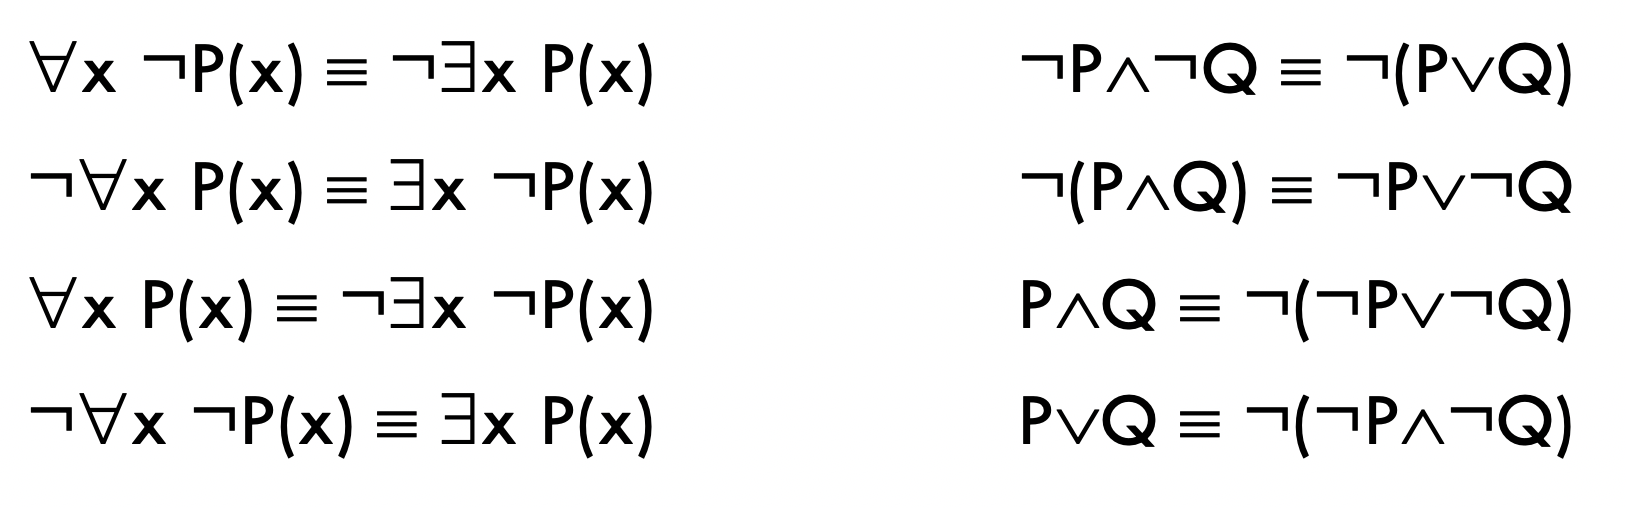
\includegraphics[scale=0.3]{Images/foarallexistsrelation.png}
\caption{Relazione tra $\forall$ ed $\exists$}
\end{figure}
\subsubsection{Semantica Standard VS Semantica database}
\begin{itemize}
    \item Standard: Ci permette di inferire.
    \item Database: simboli distinti, oggetti distinti, mondo chiuso cioè tutto ciò di cui non si sa che è vero è falso, infine esistono solo gli oggetti di cui si parla
\end{itemize}
\subsection{Interazione con la KB tramite FOL}
\begin{itemize}
    \item Asserzioni: vengono aggiunte le informazioni alla KB, esempio TELL(KB, King(John)) oppure TELL(KB, $\forall x$ King(x) $\Rightarrow$ Person(x))
    \item Conseguenze logiche: ASK(KB, Person(John)) risponde si, se KB $\models$ Person(John) altro esempio è ASK(KB, $\exists$ x Person(x)) risponde con una lista di sostituzioni o legami: [\{x/John\} \{x/George\} …]
\end{itemize}
Il metodo di risoluzione per FOL si basa sulla trasformazione in forma a clausole e poi sull'unificazione. Ci sono dei casi particolari come il Backward chaining e programmazione logica o il Forward chaining e basi di dati deduttive.
\subsection{Regola di inferenza per $\forall$}
Istanziazione dell’Universale (eliminazione del $\forall$) \quad
\infer{A[g]}{
    \forall x A[x]
} \newline
dove g è un termine ground (non già presente) e A[g] è il risultato della sostituzione di g per x in A. \newline
Ad esempio: $\forall x King(x) \land Greedy(x) \Rightarrow Evil(x)$ si ottiene $ King(John) \land Greedy(John) \Rightarrow Evil(John)$
\subsection{Regola di inferenza per $\exists$}
Istanziazione dell’esistenziale (eliminazione del $\exists$) \quad 
\infer{A[k]}{
    \exists x A[x]
} \newline
se $\exists$ non compare nell’ambito di $\forall$, k è una costante nuova (costante di Skolem) es: $\exists x Padre(x,G)$ diventa Padre(k,G) altrimenti va introdotta una funzione (di Skolem) nelle variabili quantificate universalmente ad esempio $\forll x \exists y Padre(x, y)$ diventa $ \forall x Padre(x, p(x))$
\subsubsection{Riduzione a inferenza proposizionale}
Proposizionalizzazione: creare tante istanze delle formule quantificate universalmente quanti sono gli oggetti menzionati ed eliminare i quantificatori esistenziali skolemizzando. A questo punto possiamo trattare la KB come proposizionale e applicare gli algoritmi visti. Ma ci sono dei problemi? Si, le costanti sono in numero finito ma se ci sono funzioni, il numero di istanze da creare è infinito: John, Padre(John), Padre(Padre(John))... 
\subsubsection{Teorema di Herbrand} 
Se KB $\models$ A allora c'è una dimostrazione che coinvolge solo un sotto-insieme finito della KB proposizionalizzata. Si può procedere incrementalmente, iniziando col creare le istanze con le costanti, creare poi quelle con un solo livello di annidamento Padre(John), Madre(John) ed infine quelle con due livelli di annidamento Padre(Padre(John)), Padre(Madre(John))... Se KB $\nvDash$ A il processo non termina. (Semidecidibile)
\subsection{Metodo di risoluzione per il FOL}
Per trovare un metodo di risoluzione, come abbiamo fatto per il PROP, dobbiamo estendere al FOL la trasformazione in forma a clausole e dobbiamo introdurre il concetto di unificazione.
\subsubsection{Forma a clausole}
Una clausola è un insieme di letterali, che rappresenta la loro disgiunzione:
\begin{itemize}
    \item Clausola: {Letterale, ..., Letterale}
    \item Letterale: Formula-Atomica $| \neg$ Formula-Atomica
\end{itemize}
Una KB è un insieme di clausole.\newline
Teorema: per ogni formula chiusa $\alpha$ del FOL è possibile trovare in maniera effettiva un insieme di clausole FC($\alpha$) che è soddisfacibile sse $\alpha$ lo era [o insoddisfacibile sse $\alpha$ lo era].
\subsubsection{Esempio di trasformazione (passo passo)}
Esempio di trasformazione in dettaglio per la frase “Tutti coloro che amano tutti gli animali sono amati da qualcuno” \newline il nostro risultato sarà: $\forall x ( \forall y Animale(y) \Rightarrow Ama(x,y)) \Rightarrow (\exists y Ama(y, x))$
\begin{enumerate}
    \item Eliminazione delle implicazioni ($\Rightarrow$):
    \begin{itemize}
        \item A $\Rightarrow$ B diventa	$\neg A \lor B$
        \item A $\Leftrightarrow$ B diventa $(\neg A \lor B) \land (\neg B \lor A)$
    \end{itemize}
    \item Negazioni all'interno:
    \begin{itemize}
        \item $\neg \neg A$ diventa A
        \item $\neg (A \land B)$ diventa $\neg A \lor \neg B)$
        \item $\neg (A \lor B)$ diventa $\neg A \land \neg B)$
        \item $\neg \forall x A$ diventa $\exists x \neg A$
        \item $\neg \exists x A $ diventa $\forall x \neg A$
    \end{itemize}
    \item Standardizzazione delle variabili: ogni quantificatore una variabile diversa
    \item Skolemizzazione: eliminazione dei quantificatori esistenziali
    \item Eliminazione quantificatori universali: 
    \item Forma normale congiuntiva (congiunzione di disgiunzioni di letterali):
    \item Notazione a clausole
    \item Separazione delle variabili: clausole diverse, variabili diverse
\end{enumerate}
\subsubsection{Sostituzione}
Possiamo eseguire la sostituzione in un insieme finito di associazioni tra variabili e termini, in cui ogni variabile compare una sola volta sulla sinistra. Ad esempio $\{x_1/A, x_2/f(x_3), x_3/B\}$, significa che A va sostituita a $x_1$, f($x_3$) va sostituito a $x_2$ e B a $x_3$ (nota: sulla sinistra sono solo variabili)
Sia $\sigma$ una sostituzione e A un’ espressione: $A \sigma$ è l'istanza generata dalla sostituzione (delle variabili con le corrispondenti espressioni). Possiamo scriverlo anche come Subst($\sigma$, A). \newline
Esempio:
Subst(\{x/A, y/f(B), z/w\}, P(x, x, y, v)) = P(A, A, f(B), v) \newline
Subst(\{x/g(y), y/z, z/f(x)\}, Q(x, y, z)) = Q(g(y), z, f(x)) \newline
\subsubsection{Unificazione}
L'unificazione è una operazione mediante la quale si determina se due espressioni possono essere rese identiche mediante una sostituzione di termini a variabili. Il risultato è la sostituzione che rende le due espressioni identiche detta unificatore, oppure restituisce FAIL se le espressioni non sono unificabili. \newline
Ad esempio P(A, y, z) e P(x, B, z) sono unificabili con $\tau$=\{x/A, y/B, z/C\} possiamo notare come $\tau$ sia un unificatore, ma non l’unico, un altro è $\sigma$=\{x/A, y/B\}. Possiamo infine notare come $\sigma$ è più generale di $\tau$ cioè istanzia ‘meno’ variabili. Noi però vorremmo l’unificatore più generale di tutti (MostGeneralUnifier) e abbiamo un teorema che dice che l’unificatore più generale è unico, a parte i nomi delle variabili (l’ordine non conta).
\subsubsection{Algoritmo di unificazione}
L’algoritmo di unicazione prende in input due espressioni p, q e restituisce un MGU $\Sigma$ se esiste. Possiamo chiamare l'algoritmo come UNIFY(p, q)= $\Sigma$ tale che SUBST($\Sigma$, p)= SUBST($\Sigma$, q), altrimenti FAIL. L’algoritmo esplora in parallelo le due espressioni e costruisce l’unificatore strada facendo. Appena trova espressioni non unificabili fallisce. Una causa di fallimento sono sostituzioni del tipo x=f(x), cioè sostituzioni in cui x occorre già all'interno dell'espressione. Questo controllo si chiama occurr check e in tal caso FAIL. (È un controllo di complessità quadratica)
\subsection{Esempi}
Esempio 1
\begin{itemize}
    \item UNIFY(P(A, y, z), P(x, B, z), \{\})
    \item UNIFY((A, y, z), (x, B, z), UNIFY(P, P, \{\}))
    \item UNIFY((A, y, z), (x, B, z), \{ \})
    \item UNIFY((y, z), (B, z), UNIFY(A, x, \{\}))
    \item UNIFY((y, z), (B, z), UNIFY(x, A, \{\}))
    \item UNIFY((y, z), (B, z), UNIFY-VAR(x, A, \{\}))
    \item UNIFY((y, z), (B, z), \{x/A\})
    \item UNIFY((z), (z), \{y/B, x/A\})
    \item UNIFY(z, z, \{y/B, x/A\})
    \item \{y/B, x/A\}	
\end{itemize}
Esempio 2
\begin{itemize}
    \item UNIFY(P(f(x), x), P(z, z), \{\})
    \item UNIFY((f(x), x), (z, z),UNIFY(P, P, \{\}))
    \item UNIFY((f(x), x), (z, z), \{\})
    \item UNIFY((x), (z), UNIFY(f(x), z, \{\})
    \item UNIFY((x), (z), UNIFY(z, f(x), \{\}))
    \item UNIFY((x), (z), \{z/f(x)\})
    \item UNIFY-VAR(x, z, \{z/f(x)\})
    \item UNIFY(x, f(x), \{z/f(x)\})
    \item OCCUR-CHECK(x, f(x))
    \item FAIL
\end{itemize}
\subsubsection{Metodo di risoluzione per FOL}
Siamo ora in grado di definire in generale la regola di risoluzione per FOL. \newline
\begin{figure}[h!]
\centering
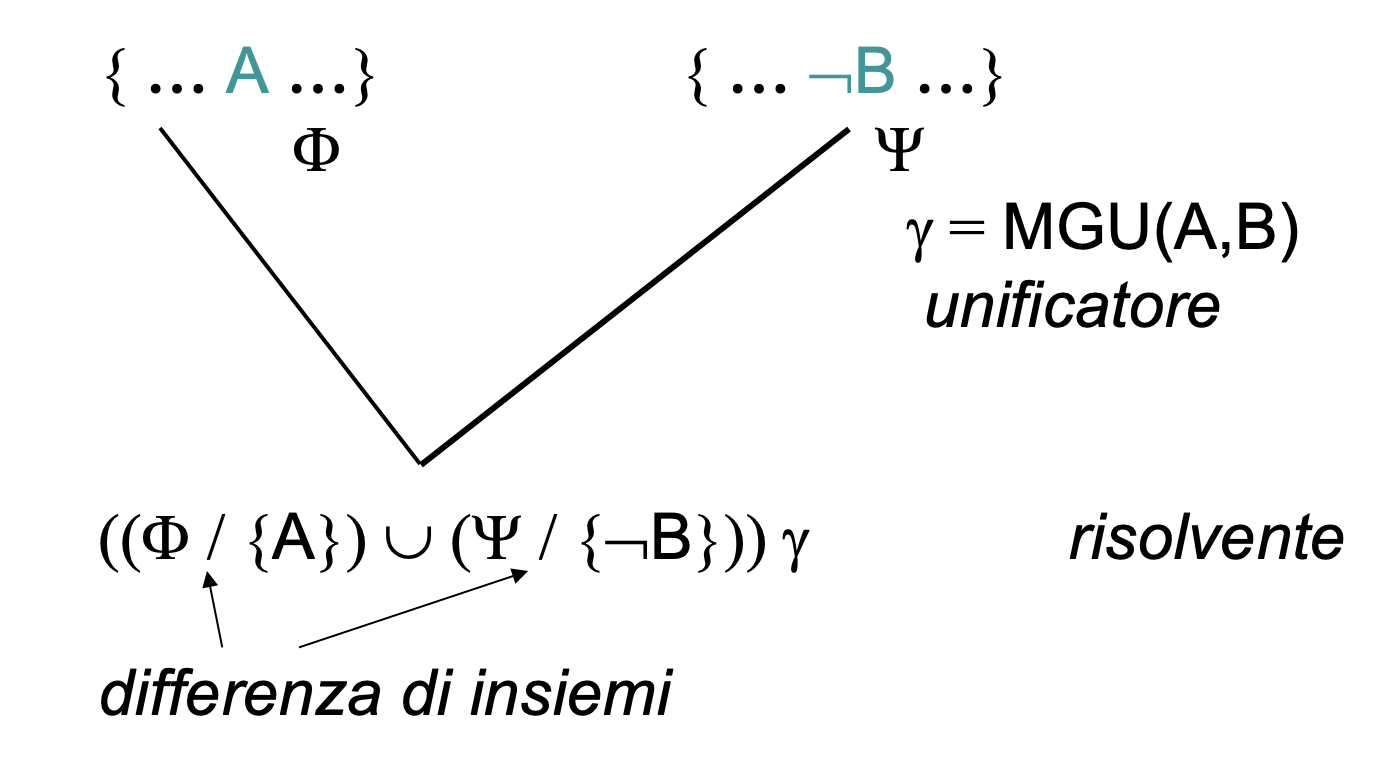
\includegraphics[scale=0.3]{Images/FOLresolmethod.png}
\end{figure}
\subsubsection{Esempio metodo di risoluzione}
\begin{figure}[h!]
\centering
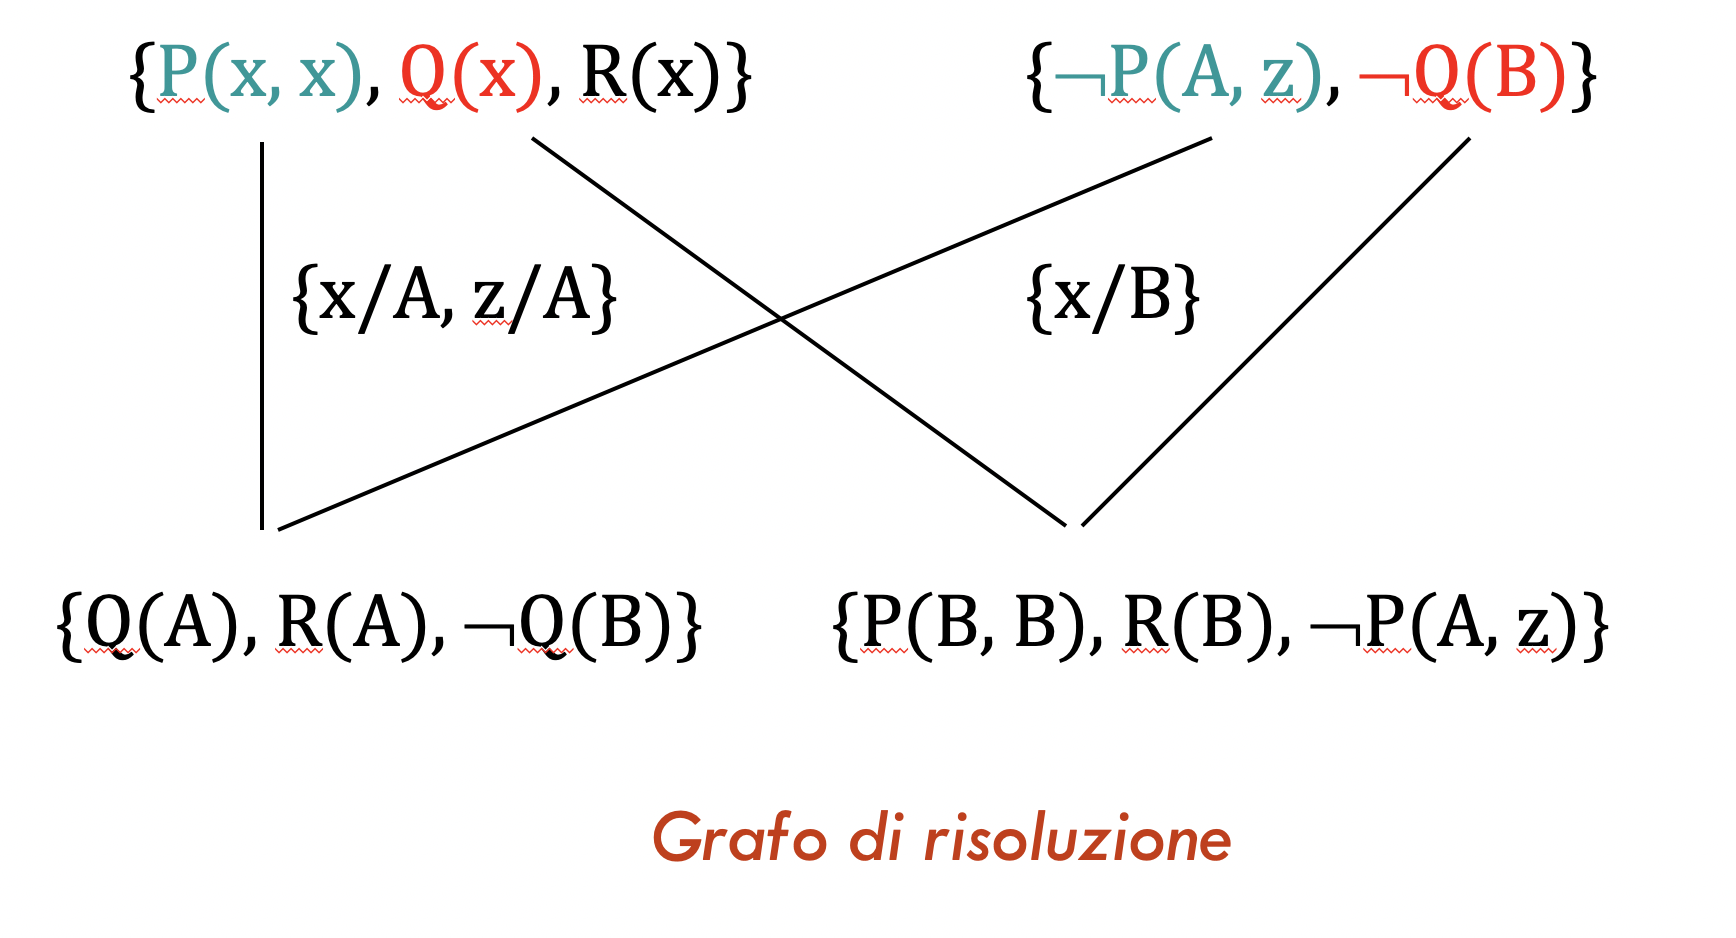
\includegraphics[scale=0.3]{Images/FOLresexample.png}
\caption{Esempio di grafo di risoluzione}
\end{figure}
\subsubsection{Problemi}
Le seguenti clausole dovrebbero produrre la clausola vuota invece...\newline
\begin{figure}[H]
\centering
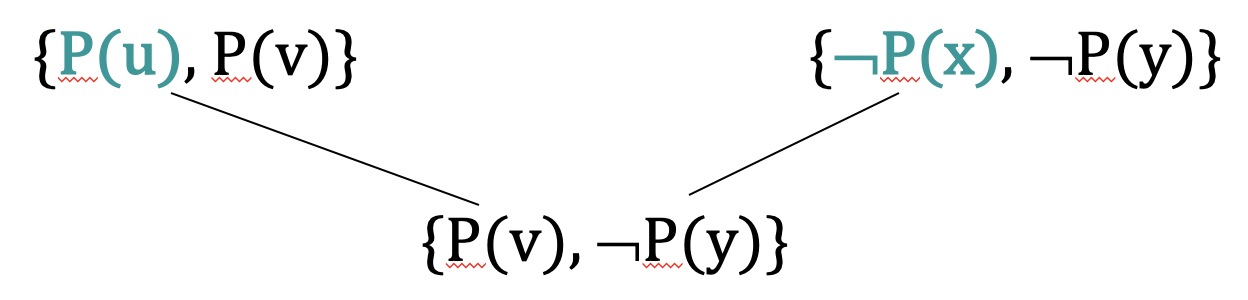
\includegraphics[scale=0.2]{Images/problem_a.png}
\end{figure}
Se un sottoinsieme dei letterali di una clausola può essere unificato allora la clausola ottenuta dopo tale unificazione si dice fattore della clausola originaria.\newline
Il metodo di risoluzione va applicato ai fattori delle clausole:
\begin{figure}[H]
\centering
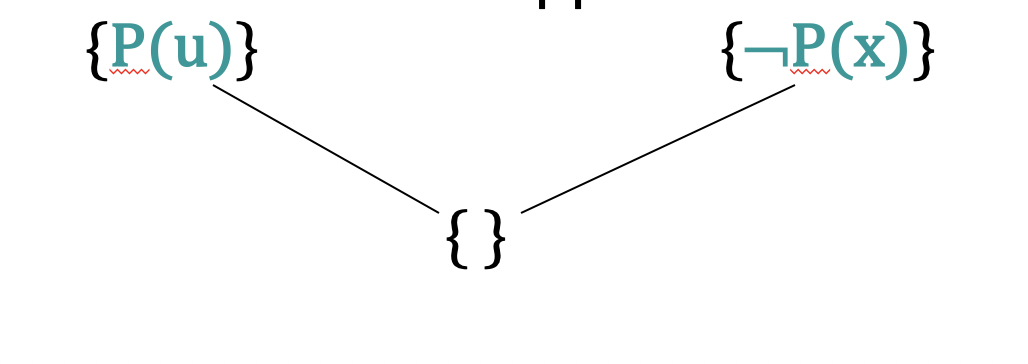
\includegraphics[scale=0.2]{Images/problem_b.png}
\end{figure}
\subsubsection{Completezza del metodo di risoluzione}
La deduzione per risoluzione è corretta	Correttezza: Se $\Gamma \vdash _{RES}$ A allora $\Gamma \models A$ \newline
La deduzione per risoluzione non è completa: può essere che $\Gamma \models A$ e non $\Gamma \vdash _{RES}$ A \newline
Un esempio è \{ \} $\models$ \{P, $\neg$P\} ma non è vero che \{ \} $\vdash _{RES}$ \{P, $\neg$P\} 
\subsubsection{Refutazione}
Come per PROP, il teorema di refutazione ci suggerisce un metodo alternativo completo. 
Il teorema di refutazione dice che $\Gamma \cup \{\neg A\}$ è insoddisfacibile sse $\Gamma \models A$. \newline
Possiamo dire quindi che $\Gamma$ è insoddisfacibile sse $\Gamma \vdash _{RES} \{\}$. Abbiamo quindi un metodo meccanizzabile, corretto e completo: basta aggiungere il negato della formula da dimostrare e provare a generare la clausola vuota.
\subsubsection{Esempio di Refutazione}
La nostra KB è formata da:
\begin{itemize}
    \item \{P(A, J)\} A è padre di J
    \item \{M(B, J)\} B è madre di J
    \item \{$\neg$P(x, y), G(x, y)\} padre implica genitore
    \item \{$\neg$M(v, w), G(v, w)\} madre implica genitore
\end{itemize} \clearpage
Il nostro goal è sapere se A è genitore di J, in forma a clausole se G(A, J) appartiene alla KB, per refutazione possiamo quindi aggiungere alla KB la negazione del goal \{$\neg$G(A, J)\} e proviamo a dedurre la clausola vuota.
\begin{figure}[H]
\centering
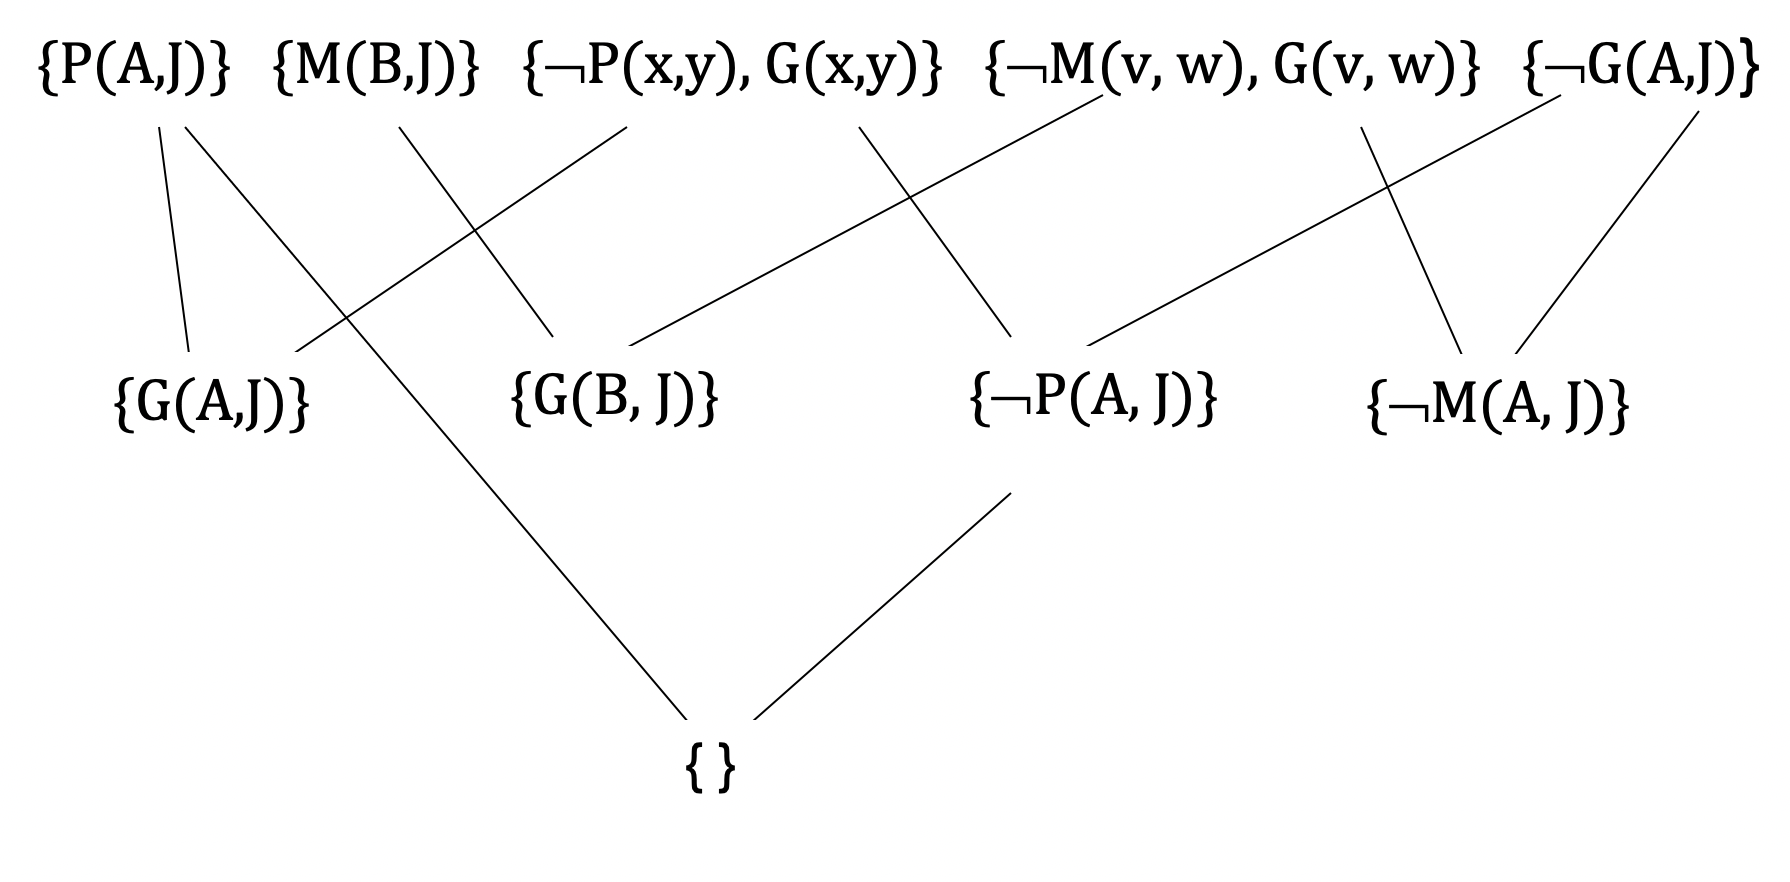
\includegraphics[scale=0.4]{Images/refutazioneesempio.png}
\end{figure}
E per domande del tipo "trova...?" come ad esempio "chi sono i genitori di J? \newline
Si cerca di dimostrare che $\exists z G(z,J) \rightarrow \{\neg G(z,J)\}$ e la risposta sono tutti i possibili legami per z che consentono di ottenere la clausola vuota.
\begin{figure}[H]
\centering
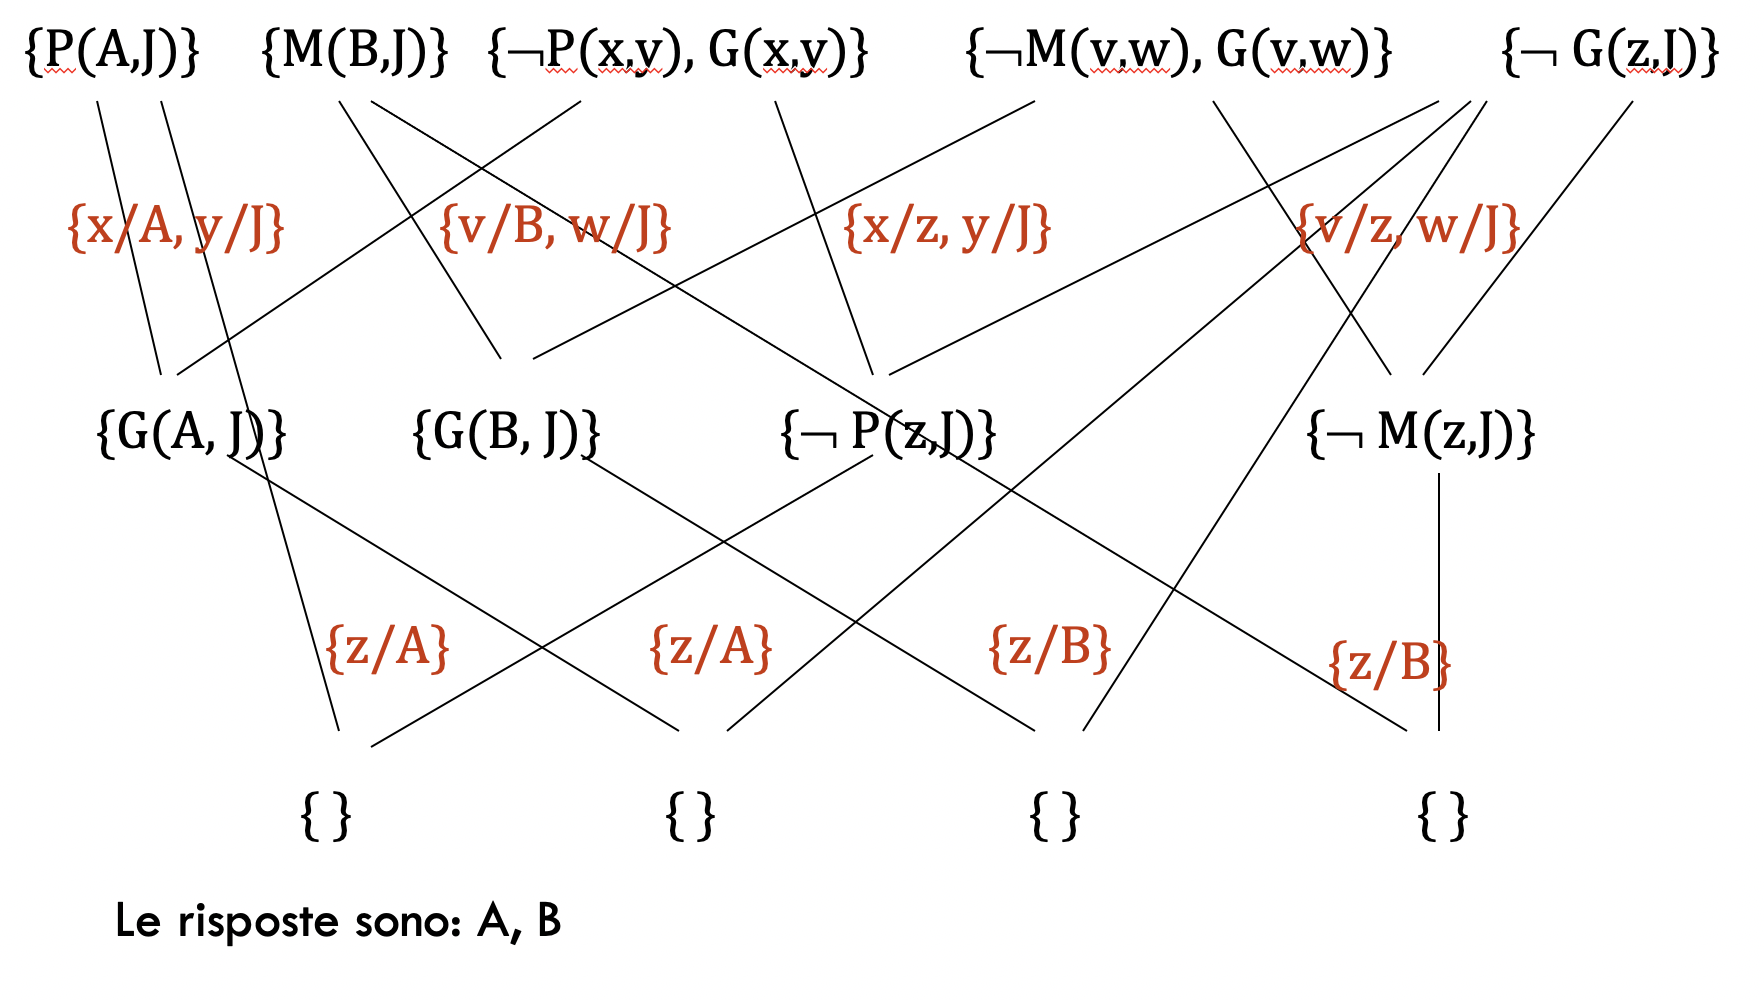
\includegraphics[scale=0.4]{Images/refutazioneesempio2.png}
\end{figure}
















%\bibliographystyle{plain}
%\bibliography{references}
\end{document}
